%% 
%% Copyright 2007, 2008, 2009 Elsevier Ltd
%% 
%% This file is part of the 'Elsarticle Bundle'.
%% ---------------------------------------------
%% 
%% It may be distributed under the conditions of the LaTeX Project Public
%% License, either version 1.2 of this license or (at your option) any
%% later version.  The latest version of this license is in
%%    http://www.latex-project.org/lppl.txt
%% and version 1.2 or later is part of all distributions of LaTeX
%% version 1999/12/01 or later.
%%
%% The list of all files belonging to the 'Elsarticle Bundle' is
%% given in the file `manifest.txt'.
%% 
%% Template article for Elsevier's document class `elsarticle'
%% with harvard style bibliographic references
%% SP 2008/03/01

\documentclass[preprint,12pt,authoryear]{elsarticle}

%% Use the option review to obtain double line spacing
%% \documentclass[authoryear,preprint,review,12pt]{elsarticle}

%% Use the options 1p,twocolumn; 3p; 3p,twocolumn; 5p; or 5p,twocolumn
%% for a journal layout:
%% \documentclass[final,1p,times,authoryear]{elsarticle}
%% \documentclass[final,1p,times,twocolumn,authoryear]{elsarticle}
%% \documentclass[final,3p,times,authoryear]{elsarticle}
%% \documentclass[final,3p,times,twocolumn,authoryear]{elsarticle}
%% \documentclass[final,5p,times,authoryear]{elsarticle}
%% \documentclass[final,5p,times,twocolumn,authoryear]{elsarticle}

%% For including figures, graphicx.sty has been loaded in
%% elsarticle.cls. If you prefer to use the old commands
%% please give \usepackage{epsfig}

%% The amssymb package provides various useful mathematical symbols
\usepackage{amssymb}
%% The amsthm package provides extended theorem environments
%% \usepackage{amsthm}

%% The lineno packages adds line numbers. Start line numbering with
%% \begin{linenumbers}, end it with \end{linenumbers}. Or switch it on
%% for the whole article with \linenumbers.
%% \usepackage{lineno}

\usepackage{url}

% Professional tables
\usepackage{booktabs}

% Rotate pages
\usepackage{pdflscape}

% Sideways table
\usepackage{rotating}

% FloatBarrier
\usepackage{placeins}

% Scientific notation of numbers
\usepackage{siunitx}
\sisetup{output-exponent-marker=\ensuremath{\mathrm{e}}}

% Subfigures
\usepackage{subcaption}

% Coloring tables
\usepackage{colortbl}
\usepackage[table*]{xcolor}
\xdefinecolor{gray95}{gray}{0.65}
\xdefinecolor{gray25}{gray}{0.8}

% ToDo Marker
\usepackage{color}
 \newcommand{\margtodo}
{\marginpar{\textbf{\textcolor{red}{ToDo}}}{}}

\newcommand{\todo}[1]
{{\textbf{\textcolor{red}{(\margtodo{}#1)}}}{}}

\journal{Applied Soft Computing}

\begin{document}

\begin{frontmatter}

%% Title, authors and addresses

%% use the tnoteref command within \title for footnotes;
%% use the tnotetext command for theassociated footnote;
%% use the fnref command within \author or \address for footnotes;
%% use the fntext command for theassociated footnote;
%% use the corref command within \author for corresponding author footnotes;
%% use the cortext command for theassociated footnote;
%% use the ead command for the email address,
%% and the form \ead[url] for the home page:
%% \title{Title\tnoteref{label1}}
%% \tnotetext[label1]{}
%% \author{Name\corref{cor1}\fnref{label2}}
%% \ead{email address}
%% \ead[url]{home page}
%% \fntext[label2]{}
%% \cortext[cor1]{}
%% \address{Address\fnref{label3}}
%% \fntext[label3]{}

\title{A Neuro-Genetic Approach for Modeling and Optimizing a Complex Cogeneration Process}

%% use optional labels to link authors explicitly to addresses:
%% \author[label1,label2]{}
%% \address[label1]{}
%% \address[label2]{}

\author[kit]{M.A. Braun}
\author[upv]{S. Seijo}
\author[upv]{J. Echanobe}
\author[kit]{P.K. Shukla}
\author[upv]{I. del Campo}
\author[kit]{H. Schmeck}

\address[upv]{Department of Electricity and Electronics, UPV/EHU, Spain}
\address[kit]{Institute AIFB, KIT, Karlsruhe, Germany}

\begin{abstract}
Cogeneration (combined Heat and Power or CHP) is the simultaneous production of electricity and useful heat with the aim of exploiting more efficiently, the energy stored in the fuel. Cogeneration is, however, a complex process that encompasses a great amount of sub-systems and variables. This fact makes it very difficult to obtain an analytical model of the whole plant and therefore providing a mechanism or a methodology able to optimize the global behavior. This paper proposes a neuro-genetic strategy for modeling and optimizing a Cogeneration Process of a Real Industrial Plant. First, the modeling of the process is carried out by means of several interconnected Neural Networks where, each Neural Network (NN) deals with a particular sub-system of the plant. Next, the obtained NN models are used by a Genetic Algorithm (GA), which solves a multiobjective optimization of the plant, where the goal is to minimize the fuel consumption and maximize both the generated electricity and the use of the heat. The proposed approach is evaluated with the data of a real cogeneration plant collected over a one-year period. Obtained results show not only that the modeling of the plant is correct but also that the optimization increases significantly the efficiency of the cogeneration plant.

\end{abstract}

\begin{keyword}
%% keywords here, in the form: keyword \sep keyword
Neural Networks \sep NSGA-II \sep Genetic Algorithm \sep Cogeneration \sep Multiobjective Optimization
%% PACS codes here, in the form: \PACS code \sep code

%% MSC codes here, in the form: \MSC code \sep code
%% or \MSC[2008] code \sep code (2000 is the default)

\end{keyword}

\end{frontmatter}

%% \linenumbers

%% main text
\section{Introduction}
\label{intro}

The process of generating electricity and useful heat at the same time is called cogeneration and is also known as combined heat and power (CHP). The ultimate goal of cogeneration is to exploit the maximum possible energy contained in a fuel. In the industry, the high temperature flue gases generated by engines, gas turbines, or other machines can be used to produce more electricity or to perform another process demanding heat. This implies cost savings because the amount of fuel required is reduced. This fuel saving also results in a reduction of pollution. These economic and environmental factors are the reasons why nowadays the number of cogeneration plants is increasing steadily. 

As many other industrial processes, CHP is a rather complex system due to a high number of variables involved, non-linear dynamics, limited analytical models and also incomplete knowledge. This fact implies that it is very troublesome to obtain a model that reproduces with fidelity the behavior of the real system. Moreover, without such a model, it becomes very difficult to carry out any formal strategy to try to optimize, in some sense, the efficiency of the process.

Soft computing (SC) algorithms provide a non-conventional way to deal with those problems characterized by their complexity, high dimensionality, hard non-linearities and vague or imprecise knowledge. Most typical soft computing algorithms are neural networks (NN), fuzzy systems (FS) and evolutionary computation (EC). Many of these techniques exhibit complementary  aspects and hence, they provide very often better performance when combined in a cooperative way rather than acting exclusively (e.g. neuro-fuzzy (NF) systems, evolutionary fuzzy (EF) systems, or neuro-evolutionary (NE) systems).

Due to those interesting properties, SC methods are widely used for modeling different industrial processes, for example, in water-treatment (\cite{Noshadi-2013}), in steel-making (\cite{Isazadeh-2012}) and paper-making industries (\cite{Zhang-2012}), or modeling boilers (\cite{Budnik-2012,Huang-2009}), among others. In addition, they are also very useful for detecting and predicting faults in industrial processes (\cite{Rakhshani-2009,Lemma-2013}) and in engines (\cite{Shatnawi-2014,Ghate-2011,Refaat-2013}). 

SC methods are also widely used in generation plants mainly for analysis/diagnosis, optimization, control or prediction purposes. Below is a summary of the more recent works, in which SC algorithms are applied in some way in CHP plants or in other similar thermal power plants.

- \textbf{NNs} are proposed in many papers for modeling one or several aspects of a CHP process, with different purposes  (see \cite{Rossi-2014} for an exhaustive bibliography revision). Some of these purposes are: 1) predicting or monitoring the power generated (\cite{De-2007,Smrekar-2010,Nikpey-2013,Sisworahardjo-2013}), the thermal efficiency and the pollutant emission (\cite{Flynn-2005,Pan-2007}) or the base-line energy (\cite{Rossi-2014}). 2) Reproducing the behavior of some plant components (\cite{Bekat-2012}). 3) Design or optimization of adaptive load-shedding models for stability (\cite{Kumar-2013}). 4) Optimization of operating parameters for plant efficiency maximization (\cite{Zomo-2011,Arslam-2011}). 5) Design of controllers (\cite{Wang-2008,Lee-2010}).

- \textbf{EC} is also utilized in many papers for optimizing different aspects of thermal power plants. A standard genetic algorithm (GA) is employed by \cite{Bertini-12} to optimize the start-up operation of a combined cycled power plant by means of a single objective function. A short optimization, also using a standard GA, is carried out by \cite{Ameri-09} for a steam power plant in which the efficiency is maximized in terms of cost and exergy. The cost of electricity generated in a combined cycle power plant is carried out by \cite{Koch-2007} by using a GA. \cite{Haja-2012} use a non-dominated sorting genetic algorithm (NSGA-II) in a two-objective optimization problem (i.e., efficiency and cost) in a steam cycle power plant. \cite{Ahmadi-2011} also use NSGA-II to tackle a two-objective function optimization (i.e. maximization of efficiency and the minimization of environmental impact) in a turbine power plant. \cite{Deb2012} solve a four-objective optimization problem of a solar thermal electricity plant using NSGA-II. \cite{Basu-11} propose to use NSGA-II for two objectives (economic and environmental) in a hydrothermal power system. 

- \textbf{FS}. FS-based techniques have also been used in thermal power plants. A fault tolerant measurement system based on Takagi-Sugeno fuzzy models for a gas turbine in a combined cycle power plant is proposed by \cite{Berrios-2011}. A Takagi-Sugeno fuzzy model of a complex parallel flow heat exchanger of a thermal plant using a fuzzy clustering technique is presented by \cite{Habi-2011}. \cite{Mazur-2009} carries out a two-objective optimization by means of a fuzzy logic for thermo-economic analysis of energy-transforming systems. \cite{Rodriguez-Martinez-2011} propose a fuzzy controller to govern the speed response of a gas turbine power plant during startup. Also, \cite{Moon-2011} propose an adaptive algorithm for dynamic matrix control (DMC) using fuzzy inference, and present its application to a drum-type boiler-turbine system in a fossil power plant. The control of a steam turbo-generators by a fully automatic fuzzy-based algorithm is presented by \cite{Gunes-2010}.

Regarding the SC Hybrid algorithms, there exist also different papers in the CHP/thermal plants context. 

- \textbf{NN+FS:} \cite{Liu2010} address the modeling of an ultra super-critical boiler system in a \SI{1000}{MW} power plant,  using fuzzy neural-network methods for controlling purposes. A neuro-fuzzy strategy is used by \cite{Bare-2005} for developing a diagnostic procedure of a cogeneration plant. In particular, the authors use NNs to model the internal combustion engines and then an FS is designed to analyze the NN outputs to detect probable system failure. An adaptive neuro-fuzzy system (i.e. ANFIS) is proposed by \cite{Mastacan-2005} to model the technological processes of a CHP plant.

- \textbf{NN+EC}: A procedure based on NN and artificial bees colony (ABC) is proposed to maximize the efficiency of a regenerative Rankine cycle with two feedwater heaters by \cite{Rashidi-2011}. Also \cite{Suresh-2011} present an NN-GA based method to optimize the efficiency of a high ash coal-fired super-critical power plant.

- \textbf{EC+FS}. A particle swarm optimization (PSO) and a fuzzy decision-making system are proposed by \cite{Sayyaadi-2011} to optimize a benchmark cogeneration system. In particular, the PSO performs a three-objective optimization process and then a final optimal solution of the Pareto frontier is selected using the fuzzy system. A swarm intelligence fuzzy clustering technique is used by \cite{Su-12} to obtain a Takagi-Sugeno fuzzy model with enhanced performance of  superheated steam temperature in a power plant. \cite{Saez-2007} propose a fuzzy predictive supervisory controller, based on genetic algorithms (GA), for gas turbines of combined cycle units.

- \textbf{EC+FS+NN}.  There even exist papers in which the three SC paradigms (i.e. NN, FS and EC) are used jointly in the CHP systems. A neuro-fuzzy system, whose parameters are trained by means of a PSO algorithm, is used by \cite{Tamiru-2009} for modeling  the steam and cooling sections of a cogeneration and cooling plant (CCP). \cite{Kwun-2007} present a neuro-fuzzy scheme, whose parameters are adjusted by means of a GA-based hybrid method, for modeling a turbine power plant. 

All the SC algorithms in the papers cited above deal with the modeling of one or more components of the plant, and/or the optimization of certain parameters of the process. However, compared with the work presented here, they are incomplete regarding some of the following issues: 1) they do not apply SC algorithms to both modeling and optimization (in fact, these are the majority); 2) the modeling process is performed often for just some components and not for the complete plant; 3) in many cases they use simulation tools or thermodynamics equations and do not work with data from a real plant; 4) optimization is carried out for a single-objective function; 5) optimization is not intended for a continuous on-line operation. These aspects can be better appreciated in Table \ref{SCmethods} where it is shown how none of the proposed methods covers all of the mentioned issues.


\begin{table}[h]
\caption{SC Applied to Cogeneration.}
\label{SCmethods} %\centering
\begin{tabular}{p{4.8cm}cccccc} \toprule
  %\hline
 Authors& Complete& Real& SC to& SC to& Multi-& On-line\\
 & plant& data& model& optimize& objective&  operation \\
 \midrule
\cite{De-2007} & $\times$ &  $\times$ &  \checkmark & $\times$ & $\times$ & $\times$ \\
\cite{Smrekar-2010} & \checkmark &  \checkmark &  \checkmark & $\times$ & $\times$ & $\times$ \\
\cite{Nikpey-2013} & $\times$ &  \checkmark &  \checkmark & $\times$ & $\times$ & $\times$ \\
\cite{Sisworahardjo-2013} & $\times$ &  $\times$ &  \checkmark & $\times$ & $\times$ & $\times$ \\
\cite{Flynn-2005} & $\checkmark$ &  $\checkmark$ &  $\checkmark$ & $\times$ & $\times$ & $\times$ \\
\cite{Pan-2007} & $\checkmark$ &  $\checkmark$ &  $\checkmark$ & $\times$ & $\times$ & $\times$ \\
\cite{Rossi-2014} & $\checkmark$ &  $\checkmark$ &  $\checkmark$ & $\times$ & $\times$ & $\times$ \\
\cite{Bekat-2012} & $\times$ &  $\checkmark$ &  $\checkmark$ & $\times$ & $\times$ & $\times$ \\
\cite{Kumar-2013} & $\checkmark$ &  $\times$ &  $\checkmark$ & $\times$ & $\times$ & $\times$ \\
\cite{Zomo-2011} & $\checkmark$  &  $\times$ &  $\checkmark$ & $\checkmark$ & $\times$ & $\times$ \\
\cite{Wang-2008} & $\times$  &  $\checkmark$ &  $\checkmark$ & $\times$ & $\times$ & $\times$ \\
\cite{Lee-2010} & $\checkmark$  &  $\checkmark$ &  $\checkmark$ & $\times$ & $\times$ & $\checkmark$\\
\cite{Bertini-12} & $\checkmark$  &  $\times$ &  $\times$ & $\checkmark$ & $\times$ & $\times$\\
\cite{Ameri-09} & $\checkmark$  &  $\times$ &  $\times$ & $\checkmark$ & $\times$ & $\times$\\
\cite{Koch-2007} & $\checkmark$  &  $\times$ &  $\times$ & $\checkmark$ & $\times$ & $\times$\\
\cite{Haja-2012} & $\checkmark$  &  $\times$ &  $\times$ & $\checkmark$ & $\checkmark$ & $\times$\\
\cite{Ahmadi-2011} & $\checkmark$  &  $\checkmark$ &  $\times$ & $\checkmark$ & $\checkmark$ & $\times$\\
\cite{Deb2012} &  $\checkmark$ &  $\times$ &  $\times$ & $\checkmark$ & $\checkmark$ & $\times$\\
\cite{Basu-11} &  $\checkmark$ &  $\times$ &  $\times$ & $\checkmark$ & $\checkmark$ & $\times$\\
\cite{Berrios-2011} &  $\checkmark$ &  $\checkmark$ &  $\checkmark$ & $\times$ & $\times$ & $\times$\\
\cite{Habi-2011} &  $\times$ &  $\checkmark$ &  $\checkmark$ & $\times$ & $\times$ & $\times$\\
\cite{Mazur-2009} &  $\checkmark$ &  $\times$ &  $\times$ & $\checkmark$ & $\checkmark$ & $\times$\\
\cite{Moon-2011} &  $\checkmark$ &  $\times$ &  $\checkmark$ & $\times$ & $\times$ & $\times$\\
\cite{Liu2010} &  $\checkmark$ &  $\checkmark$ &  $\checkmark$ & $\times$ & $\times$ & $\times$\\
\cite{Bare-2005} &  $\checkmark$ &  $\checkmark$ &  $\checkmark$ & $\times$ & $\times$ & $\times$\\
\cite{Mastacan-2005} &  $\times$ &  $\checkmark$ &  $\checkmark$ & $\times$ & $\times$ & $\times$\\
\cite{Rashidi-2011} &  $\checkmark$ &  $\times$ &  $\checkmark$ & $\checkmark$ & $\checkmark$ & $\times$\\
\cite{Suresh-2011} &  $\checkmark$ &  $\times$ &  $\checkmark$ & $\checkmark$ & $\times$ & $\checkmark$\\
\cite{Sayyaadi-2011} &  $\checkmark$ &  $\times$ &  $\times$ & $\checkmark$ & $\checkmark$ & $\times$\\
\cite{Saez-2007} &  $\times$ &  $\times$ &  $\checkmark$ & $\checkmark$ & $\times$ & $\times$\\
\cite{Kwun-2007} &  $\times$ &  $\checkmark$ &  $\checkmark$ & $\times$ & $\times$ & $\times$\\
\cite{Tamiru-2009} &  $\times$ &  $\checkmark$ &  $\checkmark$ & $\times$ & $\times$ & $\times$\\
 \bottomrule
 \end{tabular}
%\vspace{-0.3cm}
\end{table}

In this paper, we propose a global NN-EC strategy for modeling and optimizing a real CHP plant that covers all the above mentioned aspects. The modeling is made-up with several interconnected NNs, which are trained and tested with real data collected from the plant. Moreover, the modeling embraces all the process components: engines, intercoolers, steam condenser, boiler, turbine and slurry drying. The optimization process is carried out by means of a genetic algorithm and it is actually a multiobjective optimization problem, where the NNs are used to compute the values of the multiobjective function. More precisely, the goal is to simultaneously minimize the used fuel, maximize the produced electricity and maximize the useful thermal energy. In particular, we have used the ESPEA algorithm (\cite{espea}), which is a nondominated sorting type algorithm that is characterized by providing an excellent distribution of the individuals of the final population. In addition, the optimization process is fast enough to be applied in the continuous on-line process of the plant.  

The rest of the paper is organized as follows: in Section 2 the CHP plant used in the paper is described in detail. Section 3 deals with the NN-based modeling of the entire plant. Section 4 presents the GA-based multiobjective optimization process. In both these sections, the experiments carried out and the obtained results are analyzed in detail. Finally, Section 5 presents the main conclusions of the work.
\FloatBarrier
\section{CHP Plant}
\label{plant}

Fig. \ref{figplant} depicts a schematic of the CHP plant used in this paper. The plant is located in Monz\'on (Huesca), in the north of Spain\footnote{\url{http://www.energyworks.com}}. The main systems of the plant are: four internal combustion engines, four refrigeration engine circuits, an exhaust steam boiler, a steam turbine condenser, a steam turbine, and a slurry drying process. The plant produces electricity by means of the combustion engines and the steam turbine. The steam is generated with the heat contained in the exhaust gases of the four engines. Part of this heat is also used in a slurry drying process being the slurry provided by nearby farms.

\begin{figure}
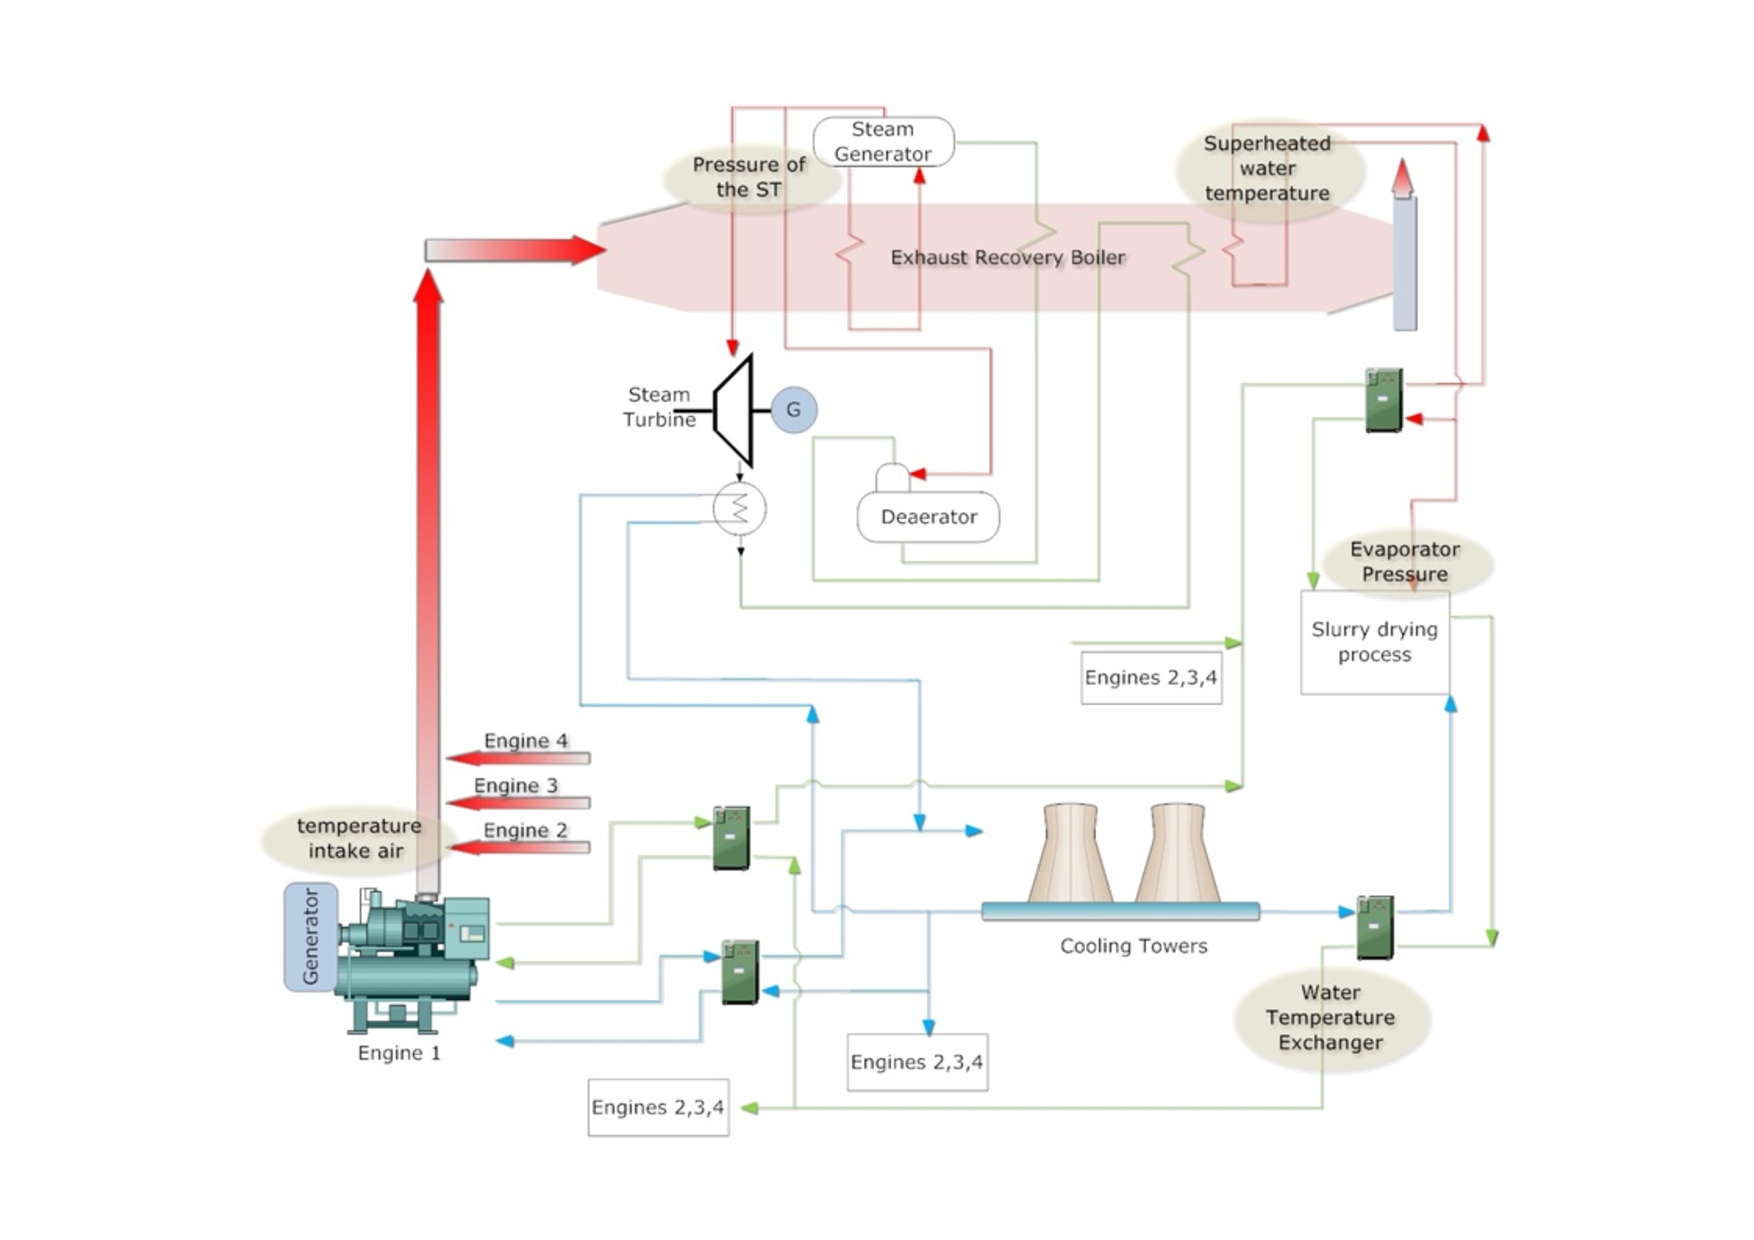
\includegraphics[width=1\textwidth]{plant.pdf}
\caption{Scheme of the combined heat and power process with their related equipment}
\label{figplant}
\end{figure}

The four internal combustion engines are all identical, with the same characteristics and the nominal power of each being \SI{3700}{kW}. They are organized into two banks with eight cylinders each and the fuel used for the combustion is natural gas. The engines exchange heat with two circuits that use water from the cooling towers, as Fig. 1 shows. A cooling circuit refrigerates the mixture of air-fuel around \SI{50}{\celsius} and the other circuit preheats the intake air to around \SI{35}{\celsius}. The engines generate electrical energy, which is sold,  and also flue gases. Each engine has a diverter which sends the flue gases to an exhaust steam boiler when the engine is working above \SI{50}{\percent} of rated power, or to the chimney if the rated power is below \SI{50}{\percent}. Engines are usually above this threshold, and therefore the flue gases go to the exhaust steam boiler most of the time. 

Next, the heat from the exhaust steam boiler is used by the steam generator to create steam around \SI{400}{\celsius} at \SI{22.5}{bar}. This steam feeds the steam turbine to generate more electricity, with \SI{1000}{kW} of nominal power. The condenser of the steam turbine uses water from the cooling towers to condensate the steam from the steam turbine and recirculate it to the system. In addition, as in the engines, the power generated for the steam turbine is also sold. 

The slurry from the farms consists of \SI{6}{\percent} solids approximately. Firstly, a mechanical treatment is carried out to remove the solid part from the rest using rotatory equipment. Then, a chemical treatment in the liquid part is performed to remove the chemical load. After that, the heat treatment uses the result of the chemical treatment to separate the condensables from non-condensables in an evaporator using superheated water generated in the exhaust steam boiler (water with a temperature around \SI{120}{\celsius}). A tubular heater is used to recirculate the effluent to the evaporator and preheat it. The tubular heater uses water from the refrigeration circuit which preheats the intake air of the engines. The non-condensable part goes with the solid part resulting from the mechanical treatment and is sold as fertilizer. The condensable effluent is condensed again with the water from the cooling towers. Finally, the sterilizer uses the heat from the superheated water to purify the condensed effluent, thereby obtaining water suitable for irrigation. 
\section{Neural Network Modeling}
\label{NN}

As it has been stated in the introduction, the modeling of the CHP plant described in the previous section has been performed by means of  NNs. In particular, we have adopted a divide-and-conquer strategy. That is, we have modeled each main component of the plant separately with an NN, and then, we have linked (connected) all the networks by means of shared or common variables (e.g.; an output variable of a network can be an input variable of one or several other networks). The global model is shown in Table \ref{fignns} where a total of twelve NNs are depicted: four for the engines, four for the engine cooling  circuits, one for the exhaust steam boiler, one for the steam turbine condenser, one for the steam turbine and finally another one for the slurry drying process. 

As neural network model, we have selected the well-known multilayer perceptron (MLP) due to its structural flexibility, good representational capabilities and availability of a large number of training algorithms (for example the Back-Propagation algorithm which is the one used here) [Haja2012]. In fact, MLP is an universal approximator and hence it is capable of approximating any measurable function to any desired degree of accuracy \cite{Hornik-1989}. It is understood, therefore, that MLP is the most common used model in those above-cited works that accomplish the modeling of cogenerations processes by means of NNs. In addition, the MLP has not a very complex structure and hence, it can be  used in a cooperative way with the evolutionary algorithm (EA) as proposed in this paper. As it will be explained in Section 4, the EA needs to evaluate the fitness function hundred of times by using the obtained NN models. A NN with a rather complex structure (e.g. recurrent NNs) would lead to a computation time too high for being used in the continuous on-line process of the plant.

In order to select the structure of the MLP model, some initial tests were made using different number of hidden layers. It was concluded that the accuracy did not show any significant improvement after increasing the number of hidden layers. Therefore, the simplest option was selected: only one hidden layer. Similarly, some initial tests were made with different number of hidden nodes. It was concluded that when the number of neurons increases beyond twice the number of inputs (i.e., a common practical rule), results barely improve. Therefore, the adopted criterion in all the models is, using twice as many hidden nodes as the number of inputs.

In our modeling,  each NN computes a single output, which in some cases becomes the input for another model (see Table \ref{fignns}).  These outputs are respectively: a) the temperature of the water to cool each engine ($T_{Mixt\_EngA}$, \dots, $T_{Mixt\_EngD}$; b) the flow of fuel (i.e. natural gas) required by each engine ($F_{Gas_A} \dots F_{Gas_D}$); c) the pressure of the condenser ($P_{CON}$); d) the steam flow in the boiler ($F_{Steam}$); e) the electric power produced by the turbine ($POW_{ST}$) and f) the flow of slurry processed by the evaporator ($F_{EV}$).

\begin{table}[!t]
\caption{CHP Neural-Networks and their corresponding variables.}
\label{fignns}
  \centering
\begin{tabular}{lll} \toprule
 Neural-Network  & Inputs of the model & Output \\ \midrule
Cooling Engine A & $\bf{T_{H2O\_Ex}}$, $T_{H2O\_TOW}, POW_A $ & $T_{Mixt\_EngA} $ \\
Cooling Engine B & $\bf{T_{H2O\_Ex}}$, $T_{H2O\_TOW}, POW_B $ & $T_{Mixt\_EngB} $ \\
Cooling Engine C & $\bf{T_{H2O\_Ex}}$, $T_{H2O\_TOW}, POW_C $ & $T_{Mixt\_EngC} $ \\
Cooling Engine D& $\bf{T_{H2O\_Ex}}$, $T_{H2O\_TOW}, POW_D $ & $T_{Mixt\_EngD} $ \\

 Engine A& $\bf{T_{B1\_A}, T_{B2\_A}}$, $T_{Amb}, H_{Amb}, LHV $ & $F_{Gas\_A} $ \\
 & $T_{Bank1\_A}, T_{Bank2\_A}, T_{Mixt\_EngA}, POW_A, DIV_A $ &  \\
 
 Engine B& $\bf{T_{B1\_B}, T_{B2\_B}}$, $T_{Amb}, H_{Amb}, LHV $ & $F_{Gas\_B} $ \\
 & $T_{Bank1\_B}, T_{Bank2\_B}, T_{Mixt\_EngB}, POW_B, DIV_B $ &  \\
 
 Engine C& $\bf{T_{B1\_C}, T_{B2\_C}}$, $T_{Amb}, H_{Amb}, LHV $ & $F_{Gas\_C} $ \\
 & $T_{Bank1\_C}, T_{Bank2\_C}, T_{Mixt\_EngC}, POW_C, DIV_C $ &  \\
 
 Engine D& $\bf{T_{B1\_D}, T_{B2\_D}}$, $T_{Amb}, H_{Amb}, LHV $ & $F_{Gas\_D} $ \\
 & $T_{Bank1\_D}, T_{Bank2\_D}, T_{Mixt\_EngD}, POW_D, DIV_D $ &  \\ 
 
Exh. steam boiler & $\bf{P_{StGen}}$, $F_{FlueGas}$ & $F_{Steam} $ \\
Steam turbine & $T_{H2O\_TOW}, T_{ST\_Cond}$ & $P_{Cond} $ \\
Condenser & & \\
Steam turbine & $P_{StGen}, F_{Steam}, P_{Cond}$ & $POW_{ST} $ \\
Slurry process & $\bf{P_{EV}, T_{H2O\_SH}, T_{H2O\_Ex}}$, $F_{Cond} $ & $F_{Ev}$ \\ \midrule


\end{tabular}
\vspace{-0.3cm}

\end{table}

To train and test the NNs, a big and complete data set was collected trough a one-year observation process in the real plant.  213 parameters were identified as being potentially relevant for training and validating the NN models. Their values have been measured and retrieved with a resolution of one minute during the whole period of observation. Firstly, a careful analysis of the data was performed to choose the most relevant variables and also to filter outliers, missing data or un-informative variables. Next, based on previous knowledge of the system physics and also on a trial/error process, we determined the particular input variables involved in each NN. Table \ref{fignns} shows which are the input/output variables for the different NNs. The variables written in bold refer to the decision variables that will be used later in the optimization process. To make the huge data set more tractable, we have selected 10-minute separated values. This action can be realized, because we have observed that the variables change very little in that period, due to the slow dynamics of the plant. We, thus, obtain a total of about \num{40000} samples for each variable. Now, for making the NNs capable of modeling the different dynamics of the process throughout the whole year, we have made the training/testing partition in the following way: data from odd months (i.e., January, March, May, \dots) are used to train the models, and data from even months (i.e., February, April, June, \dots) are used to test the modeling performance of the trained NNs. The whole training/testing process has been carried out by using the Optibat trainer Tool \cite{Optibat}.

%\begin{figure}
%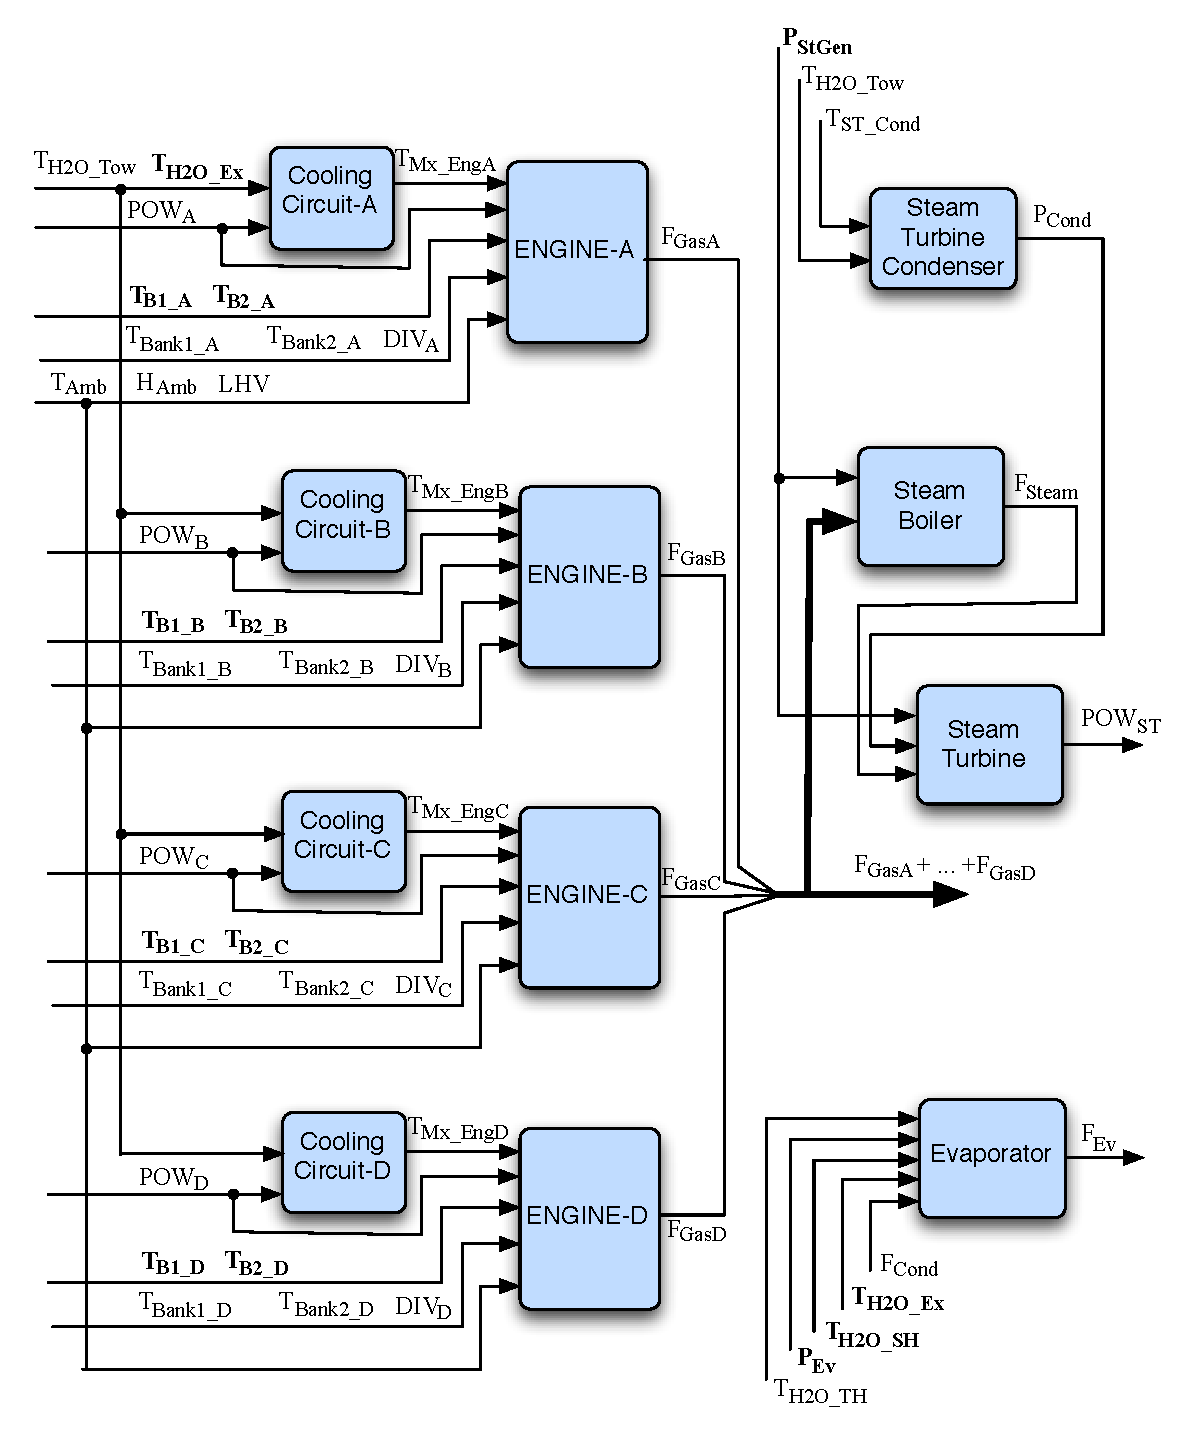
\includegraphics[width=1\textwidth]{NNs.pdf}
%\caption{Modeling of the CHP Plant by means of interconnected NNs. Each block represents an NN.}
%\label{fignns}
%\end{figure}

The results of the modeling are presented in Table \ref{tbl:mse}, where the mean squared error (MSE) between the desired and actual output, for both the training and the testing phase, is shown. We can see that, in all the cases, the obtained  errors are very small. More precisely, most of the models provide a training error less than \SI{1}{\percent}. Even in the testing case, where the NNs deal with unseen data, the error is quite small. Note that the testing error represents the model's behavior better than the training error as it contains unseen data during the training of the models. Hence, the testing error is used to evaluate the  model's  predictive behavior. We can see that for all the models, the difference between the training error and the testing error was always less than \SI{0.3}{\percent}. This means that the models were capable of learning the dynamic of the systems and can make accurate predictions when dealing with unseen data. These results validate the modeling performance of the trained NNs. 



\begin{table}[!t]
\caption{MSE for training and testing samples for each Neural Network.}
\label{tbl:mse}
  \centering
\begin{tabular}{lrrrr} \toprule
 & Structure  & Training Error & Testing Error \\ \midrule
Cooling Engine A & 3/6/1 & \SI{0.21}{\percent} & \SI{0.23}{\percent} \\
Cooling Engine B & 3/6/1  & \SI{0.28}{\percent} & \SI{0.26}{\percent} \\
Cooling Engine C & 3/6/1  & \SI{0.10}{\percent} & \SI{0.13}{\percent} \\
Cooling Engine D & 3/6/1  & \SI{0.49}{\percent} & \SI{0.33}{\percent} \\
 Engine A & 10/20/1  & \SI{0.39}{\percent} & \SI{0.42}{\percent} \\
 Engine B & 10/20/1  & \SI{0.41}{\percent} & \SI{0.41}{\percent} \\
 Engine C & 10/20/1  & \SI{0.38}{\percent} & \SI{0.42}{\percent} \\
 Engine D & 10/20/1  & \SI{0.38}{\percent} & \SI{0.37}{\percent} \\
 Recovery Boiler & 2/4/1  & \SI{0.61}{\percent} & \SI{0.63}{\percent} \\
 Steam Condenser & 2/4/1  & \SI{1.01}{\percent} & \SI{0.96}{\percent} \\
 Steam Turbine & 3/6/1  & \SI{0.67}{\percent} & \SI{0.70}{\percent} \\
 Slurry Process & 5/10/1  & \SI{2.35}{\percent} & \SI{2.52}{\percent} \\
 \bottomrule
\end{tabular}
\vspace{-0.3cm}

\end{table}

For better appreciating the modeling ability of the NNs, we have also plotted the difference between the predicted data and the real data for the testing points (Figures \ref{TcoolA} to \ref{PEvaporator}). Because the four cooling-circuit models and the four engine models have  similar behavior, we have plotted only the output variables of six of the twelve models: $T_{Mixt\_EngA}$, $F_{GasD}$, $P_{Cond}$, $F_{Steam}$, $POW_{ST}$ and $F_{Ev}$.  We can observe in these figures how, although there exists some peaks (which in somes cases they are due to outliers or unusual values) the values of these differences are in general small. In particular the mean value of these differences is below the 0.65\% in all the cases, being the model for the $T_{Mixt\_EngA}$ the best case (0.08\%) and the model for the $F_{Ev}$ the worst case (0.65\%). Thus, it is confirmed that the NNs are able to learn rather well the dynamics of the plant.


\begin{figure}
\centering
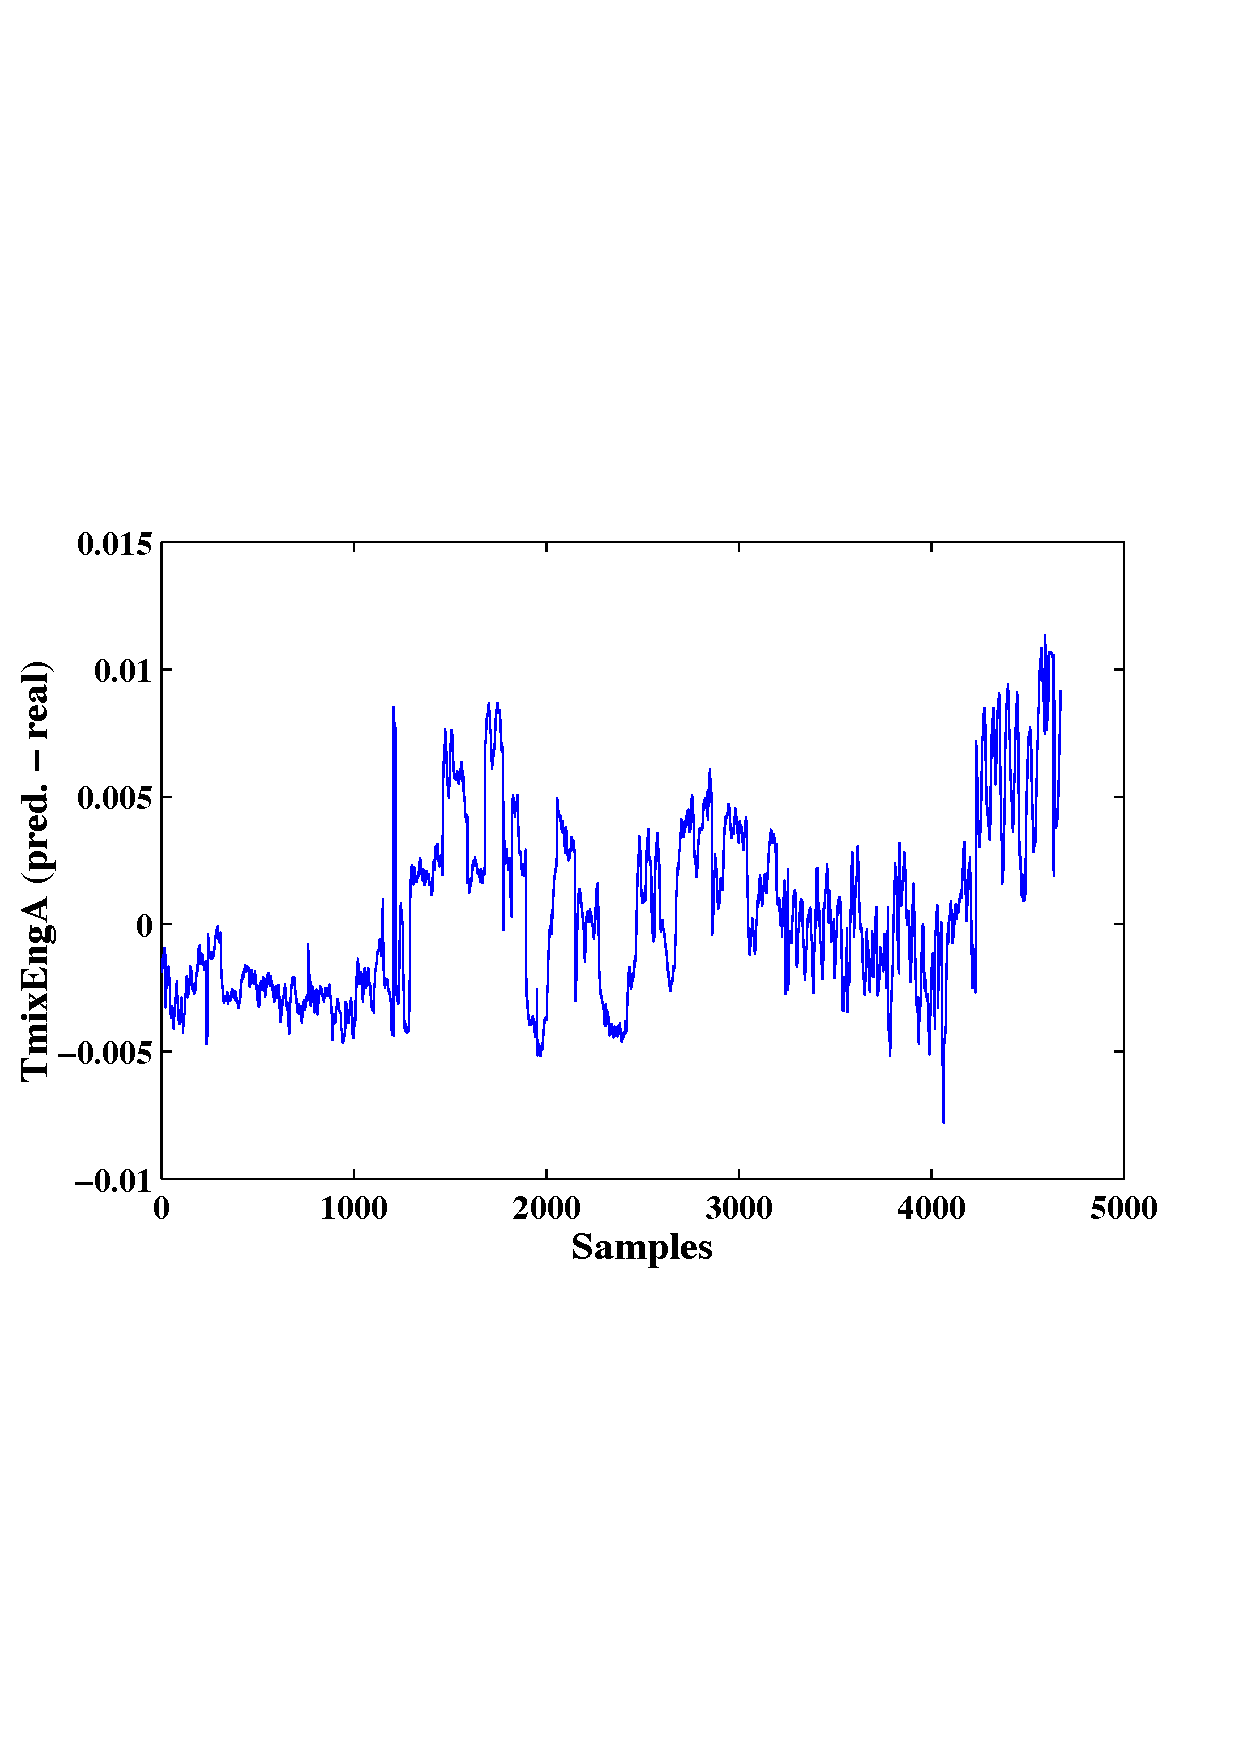
\includegraphics[width=1\textwidth]{figures/TmixEngAdiff.pdf}
\caption{Difference between real data and NN predicted data for the cooling circuit temperature of Engine A ($T_{Mixt\_EngA}$).}
\label{TcoolA}
\end{figure}

\begin{figure}
\centering
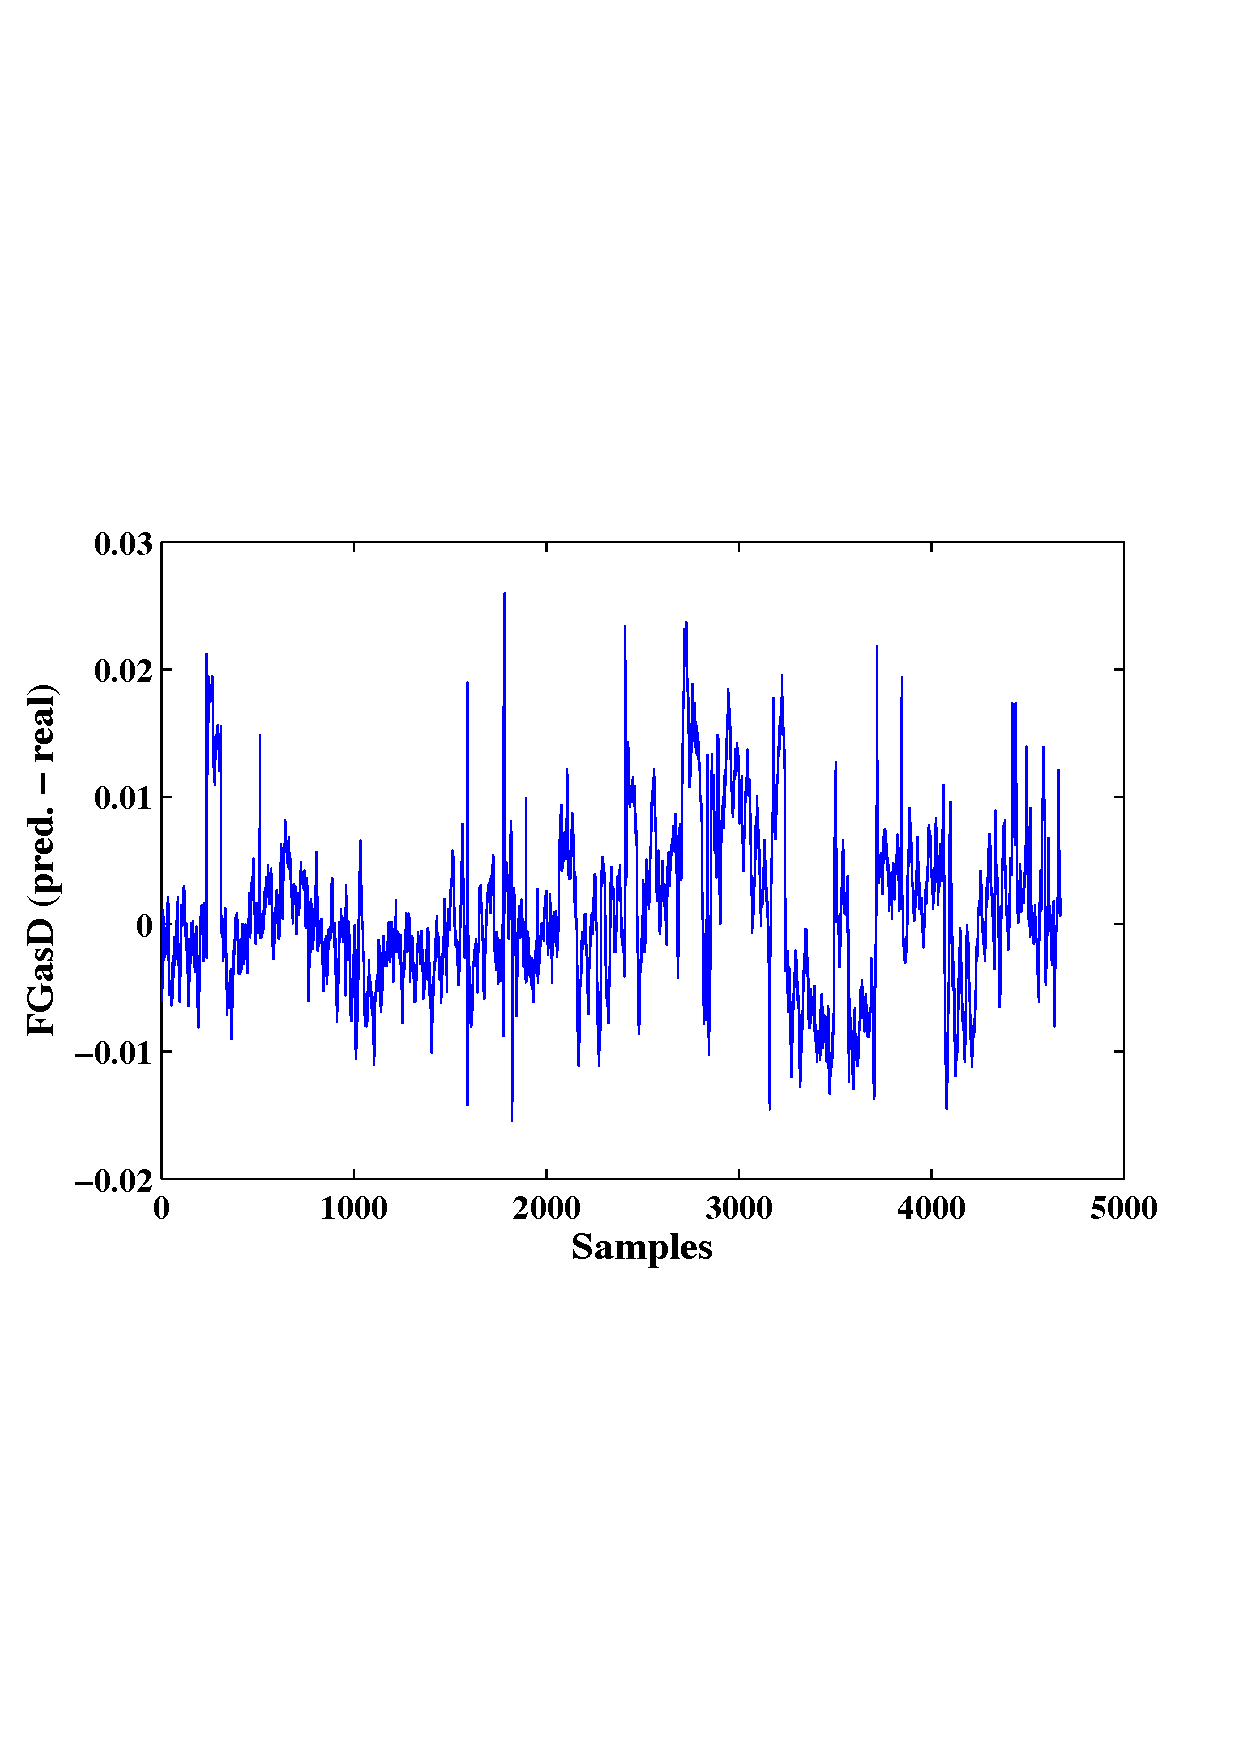
\includegraphics[width=1\textwidth]{figures/FGASDdiff.pdf}
\caption{Difference between real data and NN predicted data for the natural gas flow  of Engine A ($F_{GasA}$).}
\label{FengineA}
\end{figure}

\begin{figure}
\centering
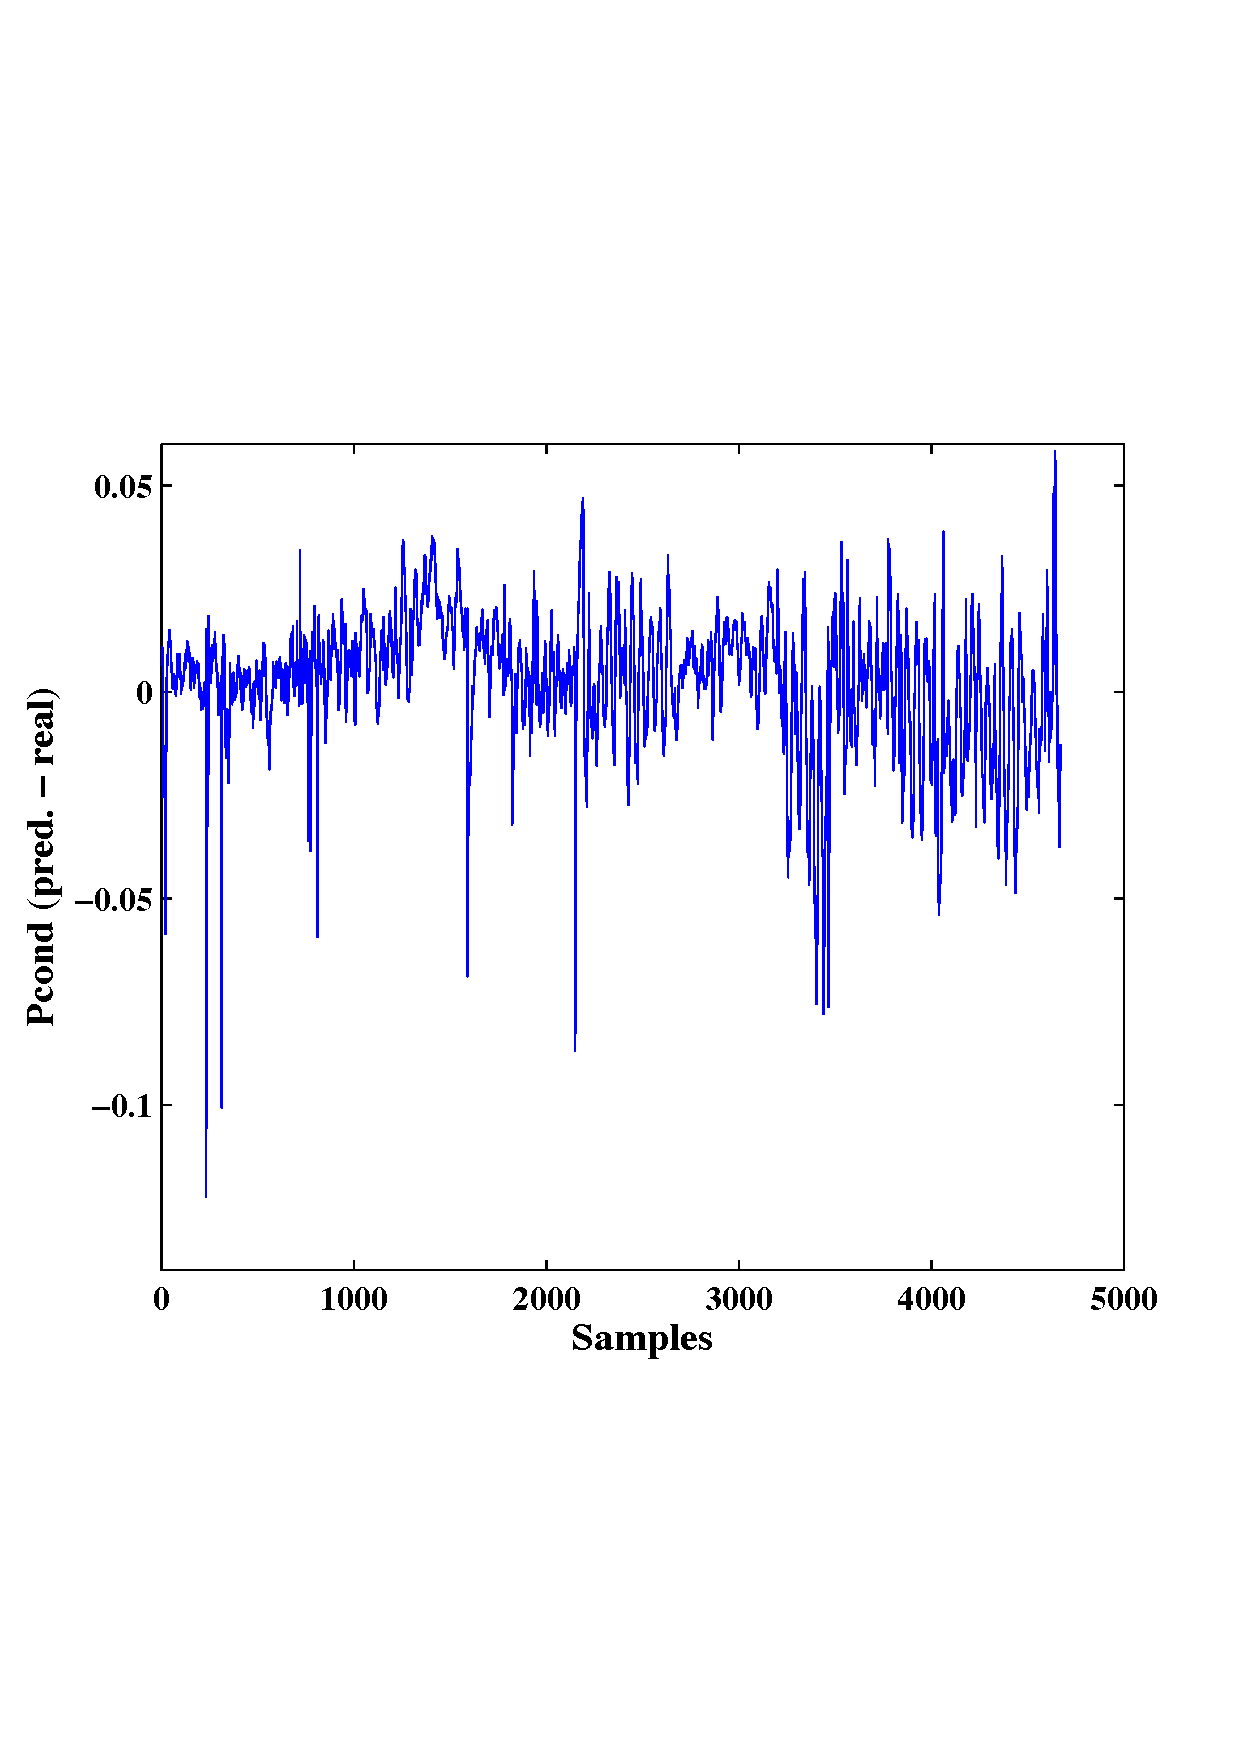
\includegraphics[width=1\textwidth]{figures/Pconddiff.pdf}
\caption{Difference between real data and NN predicted data for the steam pressure of the condenser  ($P_{Cond}$).}
\label{Pcond}
\end{figure}

\begin{figure}
\centering
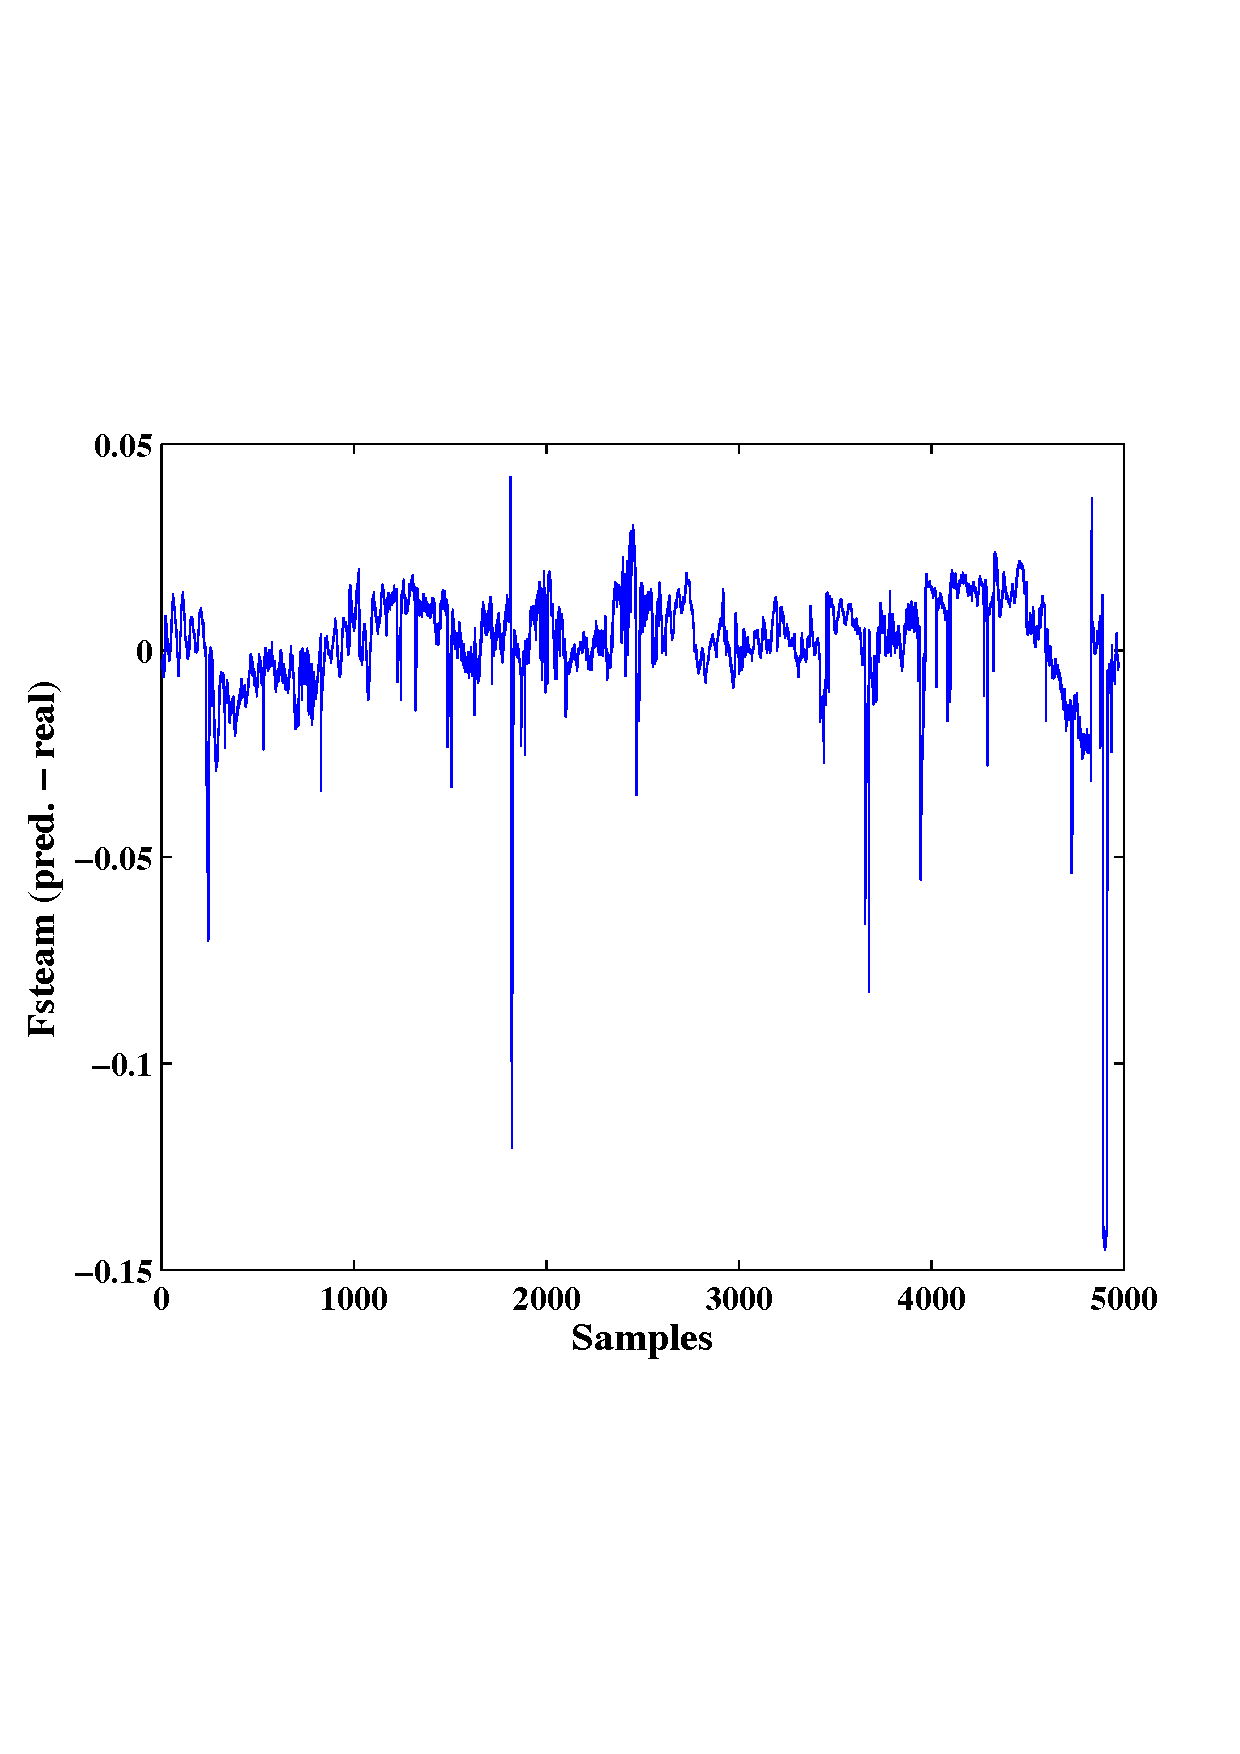
\includegraphics[width=1\textwidth]{figures/Fsteamdiff.pdf}
\caption{Difference between real data and NN predicted data for the steam flow in the boiler ($F_{Steam}$).}
\label{Fboiler}
\end{figure}

\begin{figure}
\centering
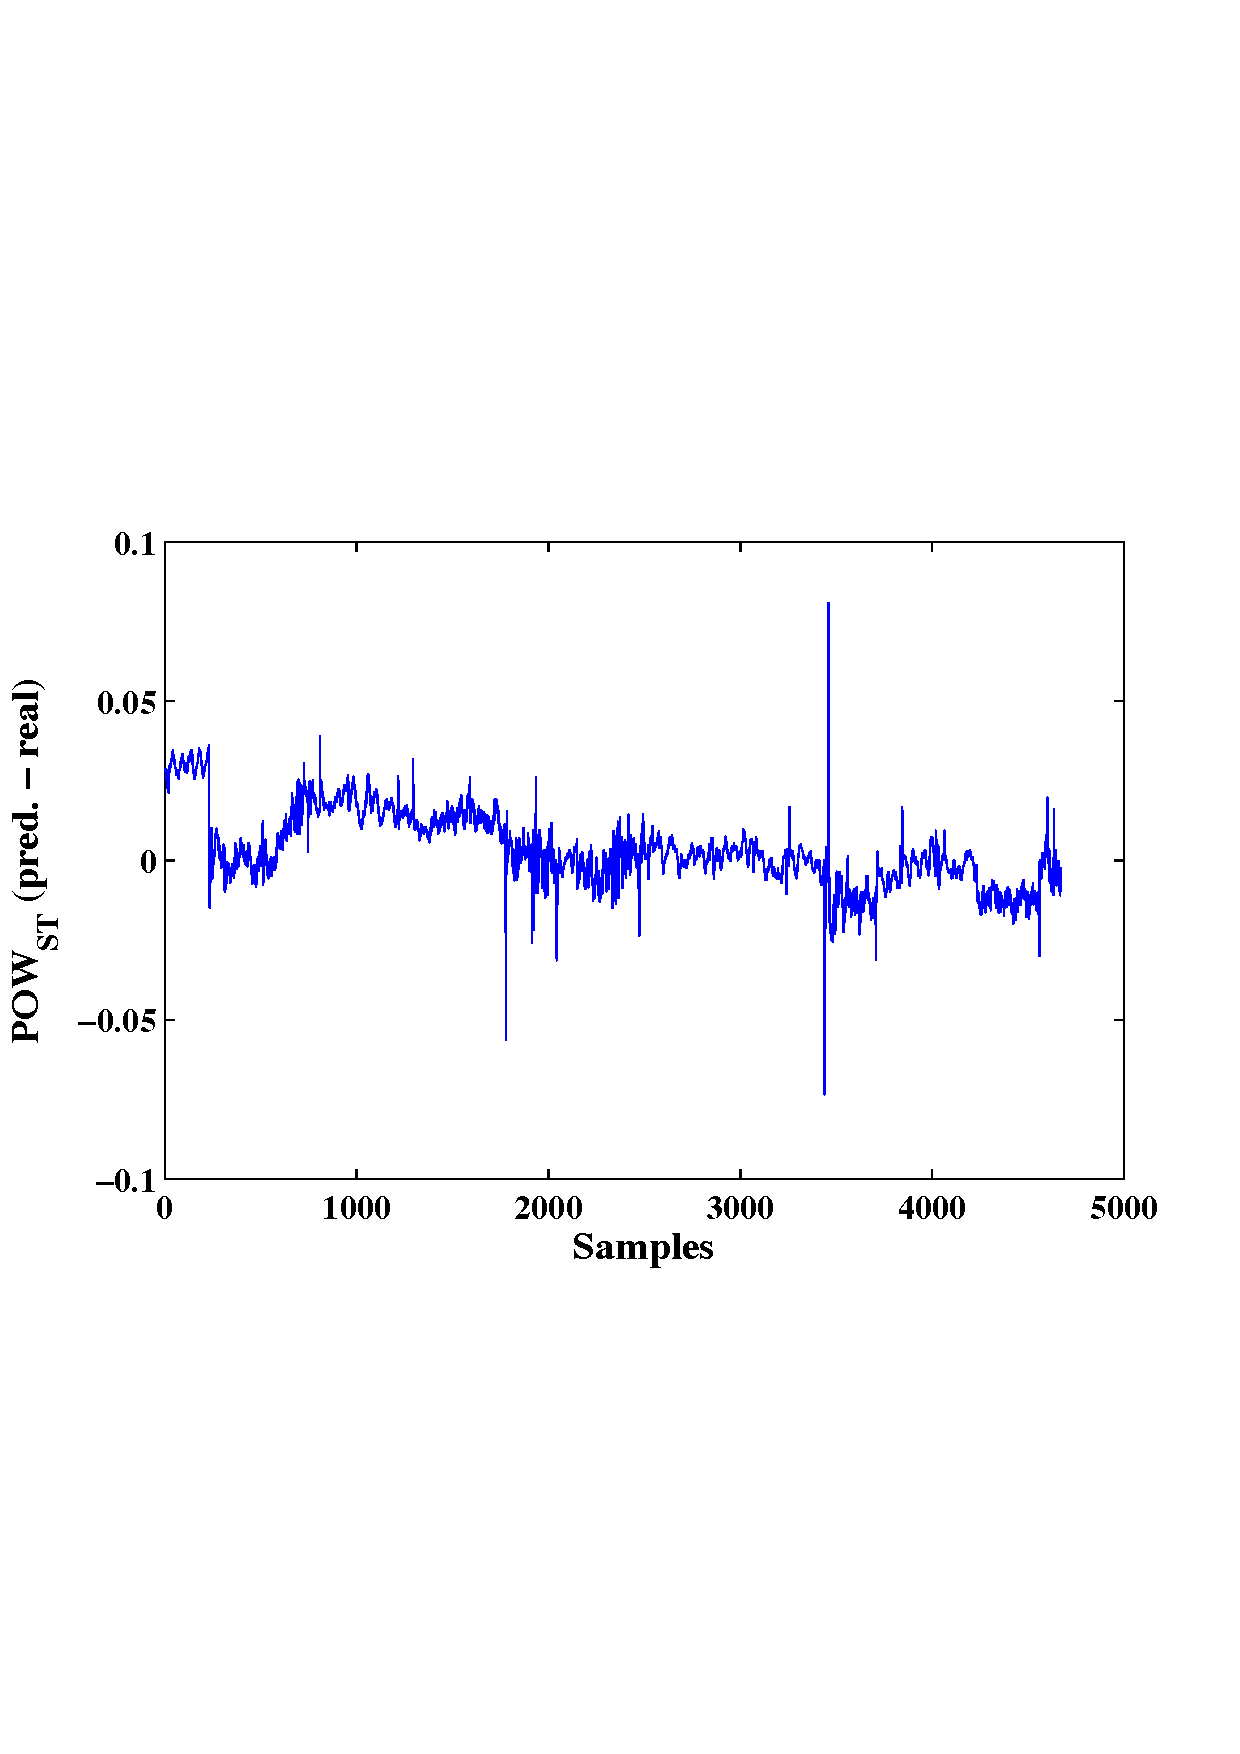
\includegraphics[width=1\textwidth]{figures/POWdiff.pdf}
\caption{Difference between real data and NN predicted data for the Power generated in the Turbine ($POW_{ST}$).}
\label{Pturbine}
\end{figure}

\begin{figure}
\centering
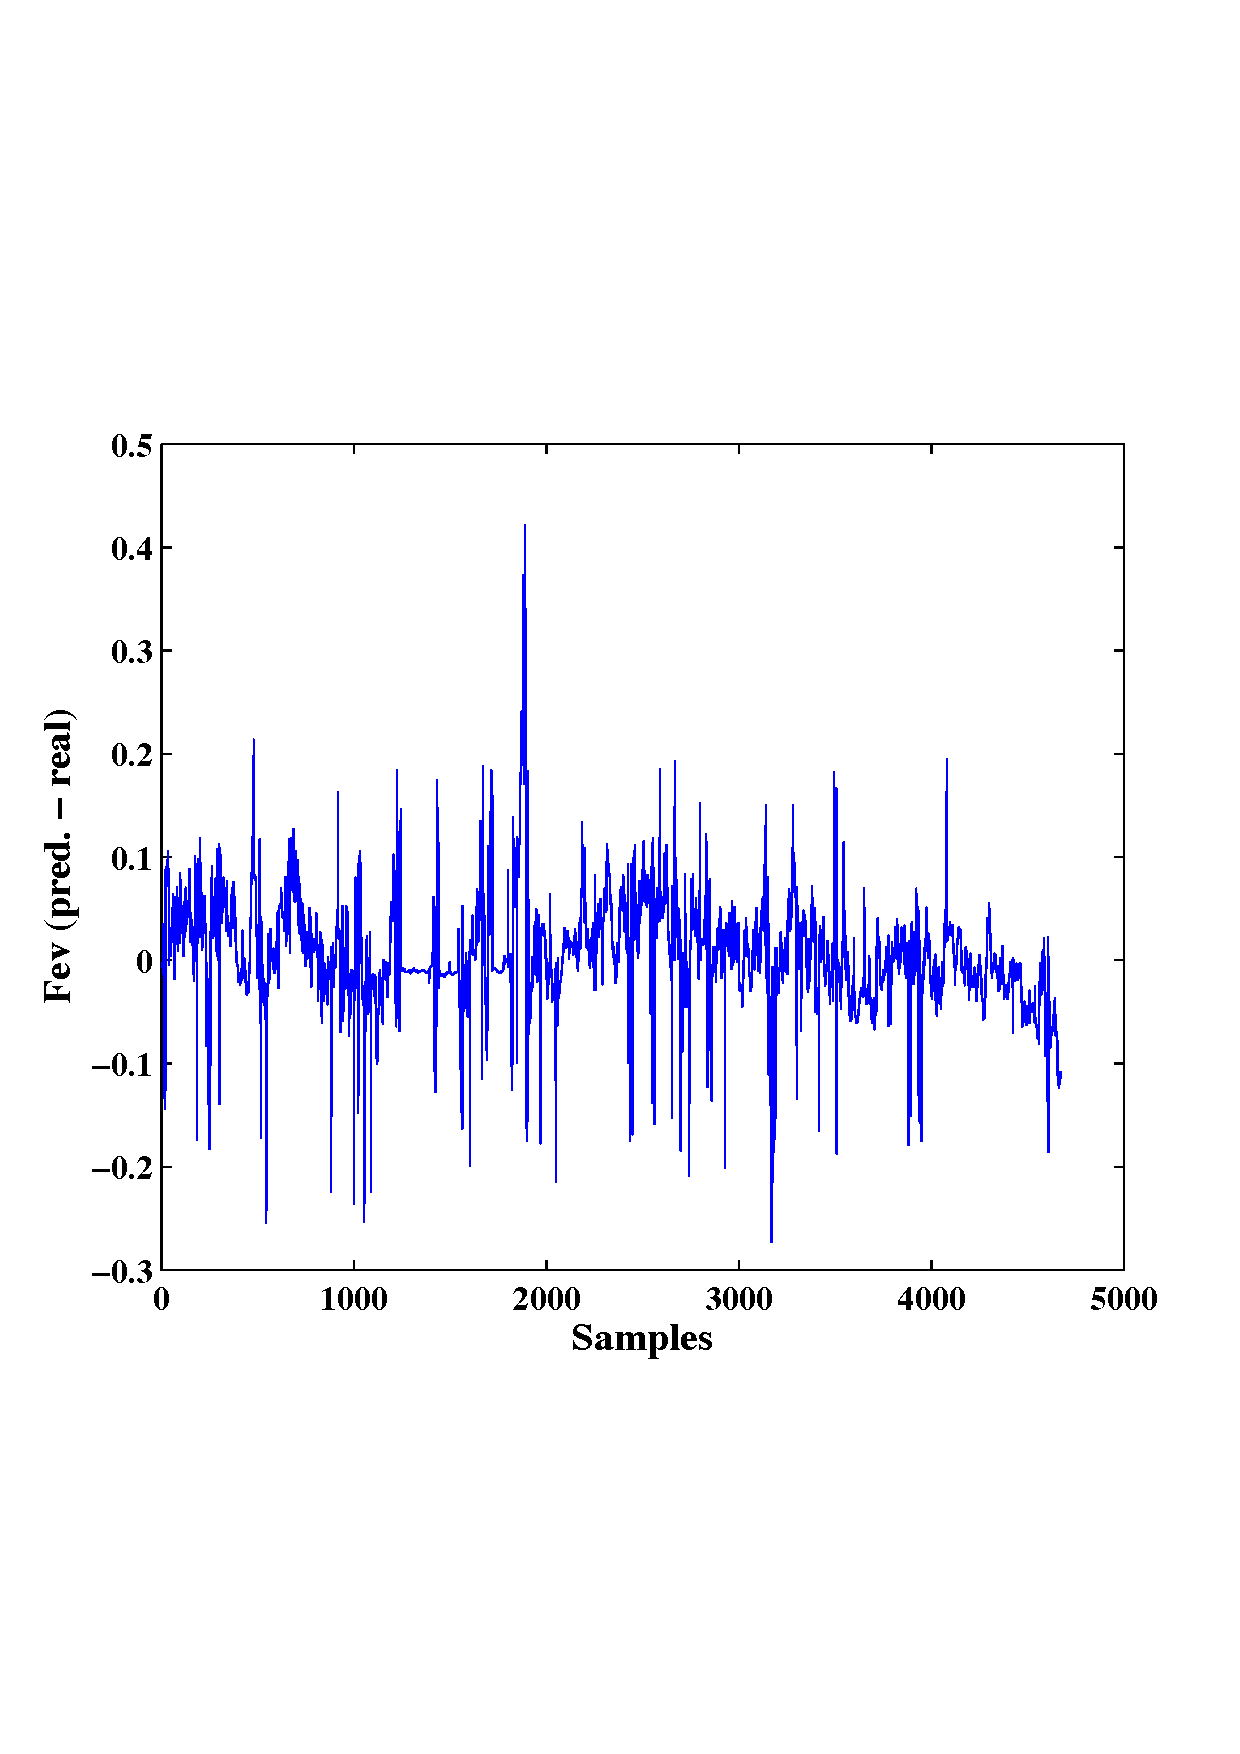
\includegraphics[width=1\textwidth]{figures/Fevdiff.pdf}
\caption{Difference between real data and NN predicted data for the Slurry drying process ($F_{Ev}$).}
\label{PEvaporator}
\end{figure}

\section{Evolutionary Algorithm-based Optimization}
\label{sec:optimization}
Once the CHP plant has been modeled by means of the connected NNs, the next step is to  carry out an optimization process to improve the efficiency of the whole process. In particular, we focus on three performance objectives: 1) to minimize the amount of used fuel FG (i.e., natural gas flow), 2) to maximize the generated power POW and 3) to maximize the useful thermal energy FEv (i.e., flow of the fluent in the evaporator). Therefore, we have actually a multi-objective optimization problem. To perform this process, a total of twelve decision variables  are available in the plant; that is, a set of input variables whose values can be changed freely (within certain limits) by the user. These twelve variables are those highlighted in  Figure  \ref{fignns}. The mathematical formulation of this multi-objective problem is as follows:
%
\begin{itemize}[-]
	\item Minimize used fuel:		$F_{FlueGas} = F_{Gas_A} + F_{Gas_B} + F_{Gas_C} + F_{Gas_D}$
	\item Maximize Power:		$POW = POW_A + POW_B + POW_C + POW_D + POW_{ST}$
	\item Maximize drying process: 	$F_{Ev}$
\end{itemize}
%
The decision variables and their restrictions are listed below:
%
\begin{itemize}[-]
	\item $T_{B1\_A}, T_{B2\_A}, T_{B1\_B}, T_{B2\_B}, T_{B1\_C}, T_{B2\_C}, T_{B1\_D}, T_{B1\_D}$. (i.e., two air intake temperatures for each engine). $30~^{\circ}\textrm{C} \leq T  \leq  38~^{\circ}\textrm{C}$
	\item $T_{H2O\_Ex}$ (exchange water temperature). $61~^{\circ}\textrm{C}  \leq T  \leq  65~^{\circ}\textrm{C}$
	\item $P_{St\_Gen}$ (pressure of the steam generator). $20~\textrm{bar}  \leq  P  \leq  22~\textrm{bar}$
	\item $P_{Ev}$ (evaporator pressure). $0.13~\textrm{bar}  \leq  P  \leq  0.17~\textrm{bar}$
	\item $T_{H2O\_SH}$ (superheated water temperature). $110~^{\circ}\textrm{C}  \leq  T  \leq  125~^{\circ}\textrm{C}$
\end{itemize}

Our combined approach of using neural networks as black box functions may be used in conjunction with any evolutionary algorithm that is able to handle real-valued decision variables. For this reason, several state-of-the-art multiobjective evolutionary algorithms are considered for solving the proposed optimization problem that all use different search strategies.

AbYSS (\cite{abyss}) uses a scatter search template as local search operator. ESPEA's (\cite{espea}) niching mechanism is based on the physical phenomenon of electrostatic potential energy. Indicator-based selection guides the search mechanism of IBEA (\cite{ibea}). MOEA/D (\cite{moead2009}) simultaneously solves multiple scalarized instances of the original problem. NSGA-II (\cite{nsga2}) uses non-dominated sorting and the crowding distance metric. It's successor, NSGA-III (\cite{nsga3part1}), uses reference point based search method. SMS-EMOA (\cite{smsemoa}) aims at finding a population that maximizes the so-called hypervolume measure. Finally, SMPSO (\cite{smpso}) is a particle swarm optimization approach.

In order to assess the performance of these individual algorithms we have performed an extensive study making use of the jMetal framework version 4.5 developed by \cite{jmetal2}. Our code and resources are hosted online on Sourceforge and are publicly available\footnote{\url{http://sourceforge.net/projects/jmetalbymarlonso/}}. The output of the cogeneration plant studied in this work is also affected by numerous external variables \todo{You have to explain to me once more, Javi, what these various configurations of the cogeneration plant mean.} that lie beyond human control. These variables, however, are observable during operation of the plant and potentially influence the performance of the evolutionary algorithm used for optimization. These different variable configurations result in several optimization scenarios that can be assessed separately. We randomly picked 39 different scenarios as representative sample for a computational study. The goal of this study is identifying the algorithm that performs best across all scenarios. Each algorithm was run 100 times on every test scenario. Algorithm configurations were taken from their original publications.

The difficulty in solving a multi-objective optimization problem is that there usually exists no single solution that optimizes all goals at the same time. Instead, optimization algorithms aim at finding a representative approximation to the so-called Pareto optimal front. The Pareto front comprises all solutions that can only be improved in one objective by impairing at least one other objective. The idea is that a decision maker chooses a solution to implement from this approximation. The approximation of a Pareto front is graded with respect to two criteria. The points found by an algorithm should be located as close as possible to the Pareto front. At the same time, the approximation should cover the Pareto front in its entirety so the decision maker has full knowledge about the available options. The former aspect is denoted by convergence and the latter by diversity.

We chose the Inverted Generational Distance (IGD) as performance metric, since it captures both convergence and diversity (\cite{van1998evolutionary}). The IGD metric computes the average of the Hausdorff distances of every Pareto optimal point to a given Pareto front approximation. Since the Pareto fronts are not known in our case, we use all nondominated solutions across all algorithm runs of a single problem instance as reference front. Objective values were normalized to mitigate the effect of different scalings.

A preliminary analysis has revealed that algorithm performances are very similar within the individual problem scenarios. This implies that our approach is very robust with respect to the initial configuration of the CHP \todo{I guess this most be phrased more correctly with respect to what this configurations actually are.}) For the sake of clarity, we therefore only provide a summary of the results in Table \todo{ref}. Full results are provided in the appendix in Table \ref{table:median.IGD}.

\todo{Summary statistics table}

The study results demonstrate that there exist clear performance differences between individual algorithms. Values of the IGD metric differ by a factor of ten from best to worst. This implies that the choice of algorithm greatly influences the optimization outcome. Best results are obtained using ESPEA, whereas AbYSS, NSGA-II and SMPSO show also good performances. IBEA, MOEA/D, NSGA-III and SMS-EMOA, on the hand, trail behind.

%______________ 

\todo{Discuss the study results}

\todo{Show an exemplary Pareto front (maybe including an ESPEA run)}

\todo{Introduce the cost function}

\todo{Algo results for the cost function}

\todo{ESPEA with augmentation}

\todo{TO BE COMPLETED}

%{\tt To carry out the multi-objective optimization process an Evolutionary Algorithm has been used. In particular, we have used the Electrostatic Potential Energy Evolutionary Algorithm ESPEA [Braun2015?] which is a non-dominated sorting genetic algorithm in which the function to assure the diversity of the obtained populations, is inspired in the Electrostatic Energy concept. As the authors show, the ESPEA algorithm outperforms other algorithms like for example NSGA-III etc. etc. etc. }



%____________________________________

\section{Conclusions}

%% The Appendices part is started with the command \appendix;
%% appendix sections are then done as normal sections
%% \appendix

\section{Acknowledgements}
This work has been partially funded by the Basque Government under Grant IT733-13, and the Spanish Ministry of Science and Innovation under Grant TEC2013-42286-R.


\section{Nomenclature}

$ANN$	Artificial Neural Networks 
\par $CHP$	Combined Heat and Power
\par $Div_A$	Diverter Engine A (\%)
\par $Div_B$	Diverter Engine B (\%)
\par $Div_C$	Diverter Engine C (\%)
\par $Div_D$	Diverter Engine D (\%)
\par $F_{Cond}$	Condensate effluent flow (kg/h) 
\par $F_{Ev}$	Flow feeded evaporator (kg/h) 
\par $F_{FlueGas}$	Flue gases Flow (kg/h) 
\par $F_{Gas_A}$	Flow Natural Gas Engine A (m3/h) 
\par $F_{Gas_B}$	Flow Natural Gas Engine B (m3/h) 
\par $F_{Gas_C}$	Flow Natural Gas Engine C (m3/h) 
\par $F_{Gas_D}$	Flow Natural Gas Engine D (m3/h) 
\par $F_{Steam}$	Steam flow to steam Turbine (kg/h)
\par $H_{Amb}$	Ambient Humidity (\%)
\par $LHV$	Low Heating Value (KWh/m3)
\par $P_{Cond}$	Condenser Pressure (bar)
\par $P_{Ev}$	Evaporator Pressure (bar) 
\par $POW_A$	Rated Power Engine A (\%) 
\par $POW_B$	Rated Power Engine B (\%) 
\par $POW_C$	Rated Power Engine C (\%) 
\par $POW_D$	Rated Power Engine D (\%) 
\par $POW_{ST}$	Turbine Power (kW)
\par $POW$		Total generated Power
\par $P_{St\_Gen}$	Steam Generator Pressure (bar)
\par $T_{B1\_A}$	Temp intake air Bank1 Engine A ($^{\circ}C$) 
\par $T_{B2\_A}$	Temp intake air Bank2 Engine A ($^{\circ}C$) 
\par $T_{B1\_B}$	Temp intake air Bank1 Engine B ($^{\circ}C$) 
\par $T_{B2\_B}$	Temp intake air Bank2 Engine B ($^{\circ}C$) 
\par $T_{B1\_C}$	Temp intake air Bank1 Engine C ($^{\circ}C$) 
\par $T_{B2\_C}$	Temp intake air Bank2 Engine C ($^{\circ}C$) 
\par $T_{B1\_D}$	Temp intake air Bank1 Engine D ($^{\circ}C$) 
\par $T_{B2\_D}$	Temp intake air Bank2 Engine D ($^{\circ}C$) 
\par $T_{Bank1\_A}$	Temp gases bank1 Engine A ($^{\circ}C$) 
\par $T_{Bank2\_A}$	Temp gases bank2 Engine A ($^{\circ}C$) 
\par $T_{Bank1\_B}$	Temp gases bank1 Engine B ($^{\circ}C$) 
\par $T_{Bank2\_B}$	Temp gases bank2 Engine B ($^{\circ}C$) 
\par $T_{Bank1\_C}$	Temp gases bank1 Engine C ($^{\circ}C$) 
\par $T_{Bank2\_C}$	Temp gases bank2 Engine C ($^{\circ}C$) 
\par $T_{Bank1\_D}$	Temp gases bank1 Engine D ($^{\circ}C$) 
\par $T_{Bank2\_D}$	Temp gases bank2 Engine D ($^{\circ}C$) 
\par $T_{H2O\_Ex}$	Water Temperature Exchange ($^{\circ}C$) 
\par $T_{H2O\_SH}$	Water Superheated Temperature ($^{\circ}C$) 
\par $T_{H2O\_TH}$	Water Temperature Tubular Heater ($^{\circ}C$) 
\par $T_{H2O\_Tow}$	Water Temperature cooling tower ($^{\circ}C$) 
\par $T_{Mixt\_EngA}$	Water Temp to cooling the Mixture Engine A ($^{\circ}C$) 
\par $T_{Mixt\_EngB}$	Water Temp to cooling the Mixture Engine B ($^{\circ}C$)  
\par $T_{Mixt\_EngC}$	Water Temp to cooling the Mixture Engine C ($^{\circ}C$)  
\par $T_{Mixt\_EngD}$	Water Temp to cooling the Mixture Engine D ($^{\circ}C$)
%% \label{}

%% If you have bibdatabase file and want bibtex to generate the
%% bibitems, please use
%%
\FloatBarrier
\bibliographystyle{elsarticle-harv} 
\bibliography{cogenBib}

\FloatBarrier
\appendix

\section{Algorithm Configurations}
\label{sec:algosetup}
Binary tournament \cite{binarytournament} selection was employed by AbYSS, IBEA, NSGA-II, NSGA-III, SMS-EMOA and ESPEA when the archive had not reached its maximum size. One selection round was performed for selecting each parent. Population members were uniformly drawn for the tournament. The winner was determined by a simple domination check. NSGA-II used crowding distance values and ESPEA energy values, IBEA fitness values and SMS-EMOA hypervolume contributions as secondary criterion if a tie occurred.

SBX crossover \cite{sbx} was used by AbYSS, IBEA, NSGA-II, NSGA-III, SMPSO, SMS-EMOA and ESPEA when the archive had not reached its maximum size. A crossover probability of 1 and a distribution index of 20 were chosen. NSGA-III used a distribution index of 30. MOEA/D and ESPEA, when the archive had reached its maximum size, used differential evolution \cite{differentialevolutionjournal}. MOEA/D used a scaling factor of 0.5 and a crossover probability of 1. ESPEA used the 'current-to-rand/1/bin' selection scheme, a crossover probability of 0.5 and a scaling factor of 0.5.

Polynomial mutation \cite{polynomialmutation} was employed by all algorithms using a mutation probability of 1 by the number of objectives and a distribution index of 20. Algorithmic-specific configurations can be found in the list below.

\begin{itemize}
	\item \textbf{AbYSS}
	\begin{itemize}
		\item population size = 20
		\item reference set 1 size = 10
		\item reference set 2 size = 10
		\item archive size = 100
	\end{itemize}
	\item \textbf{ESPEA}
	\begin{itemize}
		\item worst in archive replacement rule
		\item population size = 100
		\item archive size = 100
	\end{itemize}
	\item \textbf{IBEA}
	\begin{itemize}
		\item hypervolume indicator as fitness function
		\item population size = 100
		\item archive size = 100
	\end{itemize}
	\item \textbf{MOEA/D}
	\begin{itemize}
	  \item the same uniform weight vectors as in \cite{moead2009} were chosen
		\item population size = 100
		\item neighborhood size $T$ = 100
		\item neighborhood selection probability $\delta$ = 0.9
	\end{itemize}
	\item \textbf{NSGA-II}
	\begin{itemize}
		\item population size = 100
	\end{itemize}
	\item \textbf{ NSGA-III}
	\begin{itemize}
		\item we used the method in \cite{nbi} as suggested in \cite{nsga3part1} with 13 divisions to create 105 uniformly spread reference points
		\item population size = 100
	\end{itemize}
	\item \textbf{SMPSO}
	\begin{itemize}
		\item population size = 100
	\end{itemize}
	\item \textbf{SMS-EMOA}
	\begin{itemize}
		\item population size = 100
	\end{itemize}
\end{itemize}

%\begin{table}
%\caption{Algorithm configurations used in the computational Study.}
%\label{tbl:configs}
%\centering
%\begin{tabular}{ll} \toprule
%AbYSS & population size: 20 \\
%& reference set 1 size: 10 \\
%& reference set 2 size: 10 \\
%& archive size: 100 \\
%\end{tabular}
%\end{table}

\section{Detailed Study Results}

%\begin{landscape}
\begin{sidewaystable}
\caption{IGD. Medians and inter-quartile ranges across all 100 algorithm runs. Best and second best performances are colored in dark and light gray, respectively.}
\label{table:median.IGD}
\begin{scriptsize}
\centering
\begin{tabular}{lllllllll}
\toprule & ESPEA & AbYSS & IBEA & MOEA/D & NSGA-II & NSGA-III & SMPSO &  SMS-EMOA\\
\midrule
CG0 & \cellcolor{gray95}$  2.86e-04_{ 2.7e-06}$ & $  4.68e-04_{ 5.4e-05}$ & \cellcolor{gray25}$  3.86e-04_{ 7.7e-08}$ & $  4.67e-04_{ 6.1e-06}$ & $  4.85e-04_{ 5.5e-05}$ & $  4.62e-04_{ 1.0e-04}$ & $  4.54e-04_{ 5.2e-05}$ & $  5.14e-04_{ 1.2e-05}$ \\
CG1 & \cellcolor{gray95}$  1.66e-04_{ 2.3e-06}$ & $  3.44e-04_{ 5.6e-05}$ & $  1.56e-03_{ 1.7e-08}$ & $  1.55e-03_{ 1.1e-04}$ & $  3.49e-04_{ 6.0e-05}$ & $  1.27e-03_{ 3.3e-04}$ & \cellcolor{gray25}$  3.28e-04_{ 5.3e-05}$ & $  1.57e-03_{ 4.0e-06}$ \\
CG2 & \cellcolor{gray95}$  1.66e-04_{ 2.9e-06}$ & $  3.36e-04_{ 4.9e-05}$ & $  1.56e-03_{ 1.4e-08}$ & $  1.55e-03_{ 9.5e-05}$ & $  3.50e-04_{ 5.3e-05}$ & $  1.22e-03_{ 3.0e-04}$ & \cellcolor{gray25}$  3.35e-04_{ 5.2e-05}$ & $  1.57e-03_{ 5.5e-06}$ \\
CG3 & \cellcolor{gray95}$  1.67e-04_{ 2.8e-06}$ & $  3.35e-04_{ 3.9e-05}$ & $  1.56e-03_{ 1.3e-08}$ & $  1.55e-03_{ 3.7e-05}$ & $  3.52e-04_{ 5.5e-05}$ & $  1.21e-03_{ 3.1e-04}$ & \cellcolor{gray25}$  3.21e-04_{ 4.2e-05}$ & $  1.56e-03_{ 4.4e-06}$ \\
CG4 & \cellcolor{gray95}$  1.66e-04_{ 2.1e-06}$ & $  3.35e-04_{ 6.1e-05}$ & $  1.54e-03_{ 1.1e-08}$ & $  1.53e-03_{ 4.9e-05}$ & $  3.53e-04_{ 5.9e-05}$ & $  1.26e-03_{ 3.6e-04}$ & \cellcolor{gray25}$  3.27e-04_{ 5.0e-05}$ & $  1.55e-03_{ 5.5e-06}$ \\
CG5 & \cellcolor{gray95}$  1.66e-04_{ 2.0e-06}$ & $  3.37e-04_{ 4.9e-05}$ & $  1.56e-03_{ 1.2e-08}$ & $  1.55e-03_{ 8.8e-05}$ & $  3.58e-04_{ 5.6e-05}$ & $  1.22e-03_{ 3.2e-04}$ & \cellcolor{gray25}$  3.21e-04_{ 4.6e-05}$ & $  1.57e-03_{ 4.6e-06}$ \\
CG6 & \cellcolor{gray95}$  1.66e-04_{ 2.2e-06}$ & $  3.34e-04_{ 4.5e-05}$ & $  1.56e-03_{ 1.3e-08}$ & $  1.54e-03_{ 5.1e-05}$ & $  3.46e-04_{ 5.6e-05}$ & $  1.25e-03_{ 3.2e-04}$ & \cellcolor{gray25}$  3.21e-04_{ 4.6e-05}$ & $  1.56e-03_{ 5.0e-06}$ \\
CG7 & \cellcolor{gray95}$  1.66e-04_{ 2.5e-06}$ & $  3.42e-04_{ 4.7e-05}$ & $  1.54e-03_{ 1.3e-08}$ & $  1.53e-03_{ 5.7e-05}$ & $  3.47e-04_{ 5.8e-05}$ & $  1.28e-03_{ 2.7e-04}$ & \cellcolor{gray25}$  3.25e-04_{ 4.5e-05}$ & $  1.55e-03_{ 5.2e-06}$ \\
CG8 & \cellcolor{gray95}$  1.67e-04_{ 2.7e-06}$ & $  3.36e-04_{ 5.3e-05}$ & $  1.56e-03_{ 1.2e-08}$ & $  1.54e-03_{ 9.4e-05}$ & $  3.56e-04_{ 4.8e-05}$ & $  1.33e-03_{ 3.1e-04}$ & \cellcolor{gray25}$  3.19e-04_{ 4.8e-05}$ & $  1.57e-03_{ 4.9e-06}$ \\
CG9 & \cellcolor{gray95}$  1.66e-04_{ 2.2e-06}$ & $  3.34e-04_{ 4.3e-05}$ & $  1.56e-03_{ 1.4e-08}$ & $  1.53e-03_{ 7.7e-05}$ & $  3.47e-04_{ 6.3e-05}$ & $  1.30e-03_{ 3.1e-04}$ & \cellcolor{gray25}$  3.25e-04_{ 5.0e-05}$ & $  1.56e-03_{ 5.4e-06}$ \\
CG10 & \cellcolor{gray95}$  1.66e-04_{ 2.6e-06}$ & $  3.40e-04_{ 4.6e-05}$ & $  1.56e-03_{ 1.5e-08}$ & $  1.55e-03_{ 7.2e-05}$ & $  3.57e-04_{ 6.1e-05}$ & $  1.25e-03_{ 3.1e-04}$ & \cellcolor{gray25}$  3.28e-04_{ 5.3e-05}$ & $  1.57e-03_{ 3.9e-06}$ \\
CG11 & \cellcolor{gray95}$  1.65e-04_{ 2.3e-06}$ & $  3.44e-04_{ 5.0e-05}$ & $  1.54e-03_{ 1.3e-08}$ & $  1.53e-03_{ 5.9e-05}$ & $  3.50e-04_{ 5.9e-05}$ & $  1.30e-03_{ 3.0e-04}$ & \cellcolor{gray25}$  3.34e-04_{ 4.0e-05}$ & $  1.55e-03_{ 4.0e-06}$ \\
CG12 & \cellcolor{gray95}$  1.66e-04_{ 2.1e-06}$ & $  3.41e-04_{ 5.7e-05}$ & $  1.55e-03_{ 1.2e-08}$ & $  1.53e-03_{ 8.5e-05}$ & $  3.64e-04_{ 6.1e-05}$ & $  1.25e-03_{ 2.6e-04}$ & \cellcolor{gray25}$  3.29e-04_{ 5.9e-05}$ & $  1.56e-03_{ 5.0e-06}$ \\
CG13 & \cellcolor{gray95}$  1.66e-04_{ 2.8e-06}$ & $  3.43e-04_{ 4.5e-05}$ & $  1.56e-03_{ 1.3e-08}$ & $  1.54e-03_{ 9.2e-05}$ & $  3.60e-04_{ 5.9e-05}$ & $  1.28e-03_{ 3.1e-04}$ & \cellcolor{gray25}$  3.25e-04_{ 4.4e-05}$ & $  1.57e-03_{ 4.5e-06}$ \\
CG14 & \cellcolor{gray95}$  1.66e-04_{ 2.3e-06}$ & $  3.40e-04_{ 4.7e-05}$ & $  1.56e-03_{ 1.4e-08}$ & $  1.54e-03_{ 8.4e-05}$ & $  3.50e-04_{ 6.4e-05}$ & $  1.26e-03_{ 2.9e-04}$ & \cellcolor{gray25}$  3.23e-04_{ 3.9e-05}$ & $  1.56e-03_{ 4.2e-06}$ \\
CG15 & \cellcolor{gray95}$  1.66e-04_{ 2.5e-06}$ & $  3.39e-04_{ 4.8e-05}$ & $  1.56e-03_{ 1.3e-08}$ & $  1.53e-03_{ 5.8e-05}$ & $  3.46e-04_{ 5.7e-05}$ & $  1.26e-03_{ 3.3e-04}$ & \cellcolor{gray25}$  3.22e-04_{ 4.4e-05}$ & $  1.56e-03_{ 5.1e-06}$ \\
CG16 & \cellcolor{gray95}$  1.66e-04_{ 2.4e-06}$ & $  3.34e-04_{ 3.7e-05}$ & $  1.57e-03_{ 1.5e-08}$ & $  1.55e-03_{ 6.8e-05}$ & $  3.42e-04_{ 4.7e-05}$ & $  1.30e-03_{ 2.6e-04}$ & \cellcolor{gray25}$  3.27e-04_{ 5.5e-05}$ & $  1.58e-03_{ 4.6e-06}$ \\
CG17 & \cellcolor{gray95}$  1.67e-04_{ 2.1e-06}$ & $  3.40e-04_{ 4.8e-05}$ & $  1.56e-03_{ 9.2e-09}$ & $  1.54e-03_{ 5.9e-05}$ & $  3.53e-04_{ 5.7e-05}$ & $  1.22e-03_{ 3.4e-04}$ & \cellcolor{gray25}$  3.28e-04_{ 4.5e-05}$ & $  1.56e-03_{ 4.7e-06}$ \\
CG18 & \cellcolor{gray95}$  1.66e-04_{ 2.4e-06}$ & $  3.35e-04_{ 5.0e-05}$ & $  1.55e-03_{ 1.3e-08}$ & $  1.53e-03_{ 9.7e-05}$ & $  3.47e-04_{ 5.4e-05}$ & $  1.27e-03_{ 3.6e-04}$ & \cellcolor{gray25}$  3.24e-04_{ 4.0e-05}$ & $  1.56e-03_{ 4.3e-06}$ \\
CG19 & \cellcolor{gray95}$  1.66e-04_{ 2.1e-06}$ & $  3.41e-04_{ 4.9e-05}$ & $  1.56e-03_{ 1.4e-08}$ & $  1.53e-03_{ 7.6e-05}$ & $  3.49e-04_{ 5.0e-05}$ & $  1.30e-03_{ 3.2e-04}$ & \cellcolor{gray25}$  3.31e-04_{ 5.2e-05}$ & $  1.56e-03_{ 5.3e-06}$ \\
CG20 & \cellcolor{gray95}$  1.66e-04_{ 2.8e-06}$ & $  3.38e-04_{ 5.4e-05}$ & $  1.56e-03_{ 1.6e-08}$ & $  1.55e-03_{ 8.2e-05}$ & $  3.50e-04_{ 5.2e-05}$ & $  1.28e-03_{ 3.0e-04}$ & \cellcolor{gray25}$  3.31e-04_{ 4.3e-05}$ & $  1.57e-03_{ 4.4e-06}$ \\
CG21 & \cellcolor{gray95}$  1.66e-04_{ 2.9e-06}$ & $  3.35e-04_{ 4.8e-05}$ & $  1.57e-03_{ 1.3e-08}$ & $  1.55e-03_{ 4.8e-05}$ & $  3.46e-04_{ 4.9e-05}$ & $  1.29e-03_{ 3.3e-04}$ & \cellcolor{gray25}$  3.26e-04_{ 4.4e-05}$ & $  1.57e-03_{ 3.9e-06}$ \\
CG22 & \cellcolor{gray95}$  1.66e-04_{ 2.3e-06}$ & $  3.34e-04_{ 5.3e-05}$ & $  1.55e-03_{ 1.4e-08}$ & $  1.53e-03_{ 1.0e-04}$ & $  3.51e-04_{ 4.3e-05}$ & $  1.25e-03_{ 3.6e-04}$ & \cellcolor{gray25}$  3.26e-04_{ 4.3e-05}$ & $  1.56e-03_{ 5.3e-06}$ \\
CG23 & \cellcolor{gray95}$  1.66e-04_{ 2.2e-06}$ & $  3.41e-04_{ 4.2e-05}$ & $  1.55e-03_{ 1.7e-08}$ & $  1.54e-03_{ 5.3e-05}$ & $  3.47e-04_{ 4.9e-05}$ & $  1.28e-03_{ 2.6e-04}$ & \cellcolor{gray25}$  3.27e-04_{ 4.4e-05}$ & $  1.56e-03_{ 4.6e-06}$ \\
CG24 & \cellcolor{gray95}$  1.66e-04_{ 2.0e-06}$ & $  3.32e-04_{ 5.2e-05}$ & $  1.56e-03_{ 1.7e-08}$ & $  1.53e-03_{ 1.1e-04}$ & $  3.47e-04_{ 6.4e-05}$ & $  1.28e-03_{ 2.8e-04}$ & \cellcolor{gray25}$  3.31e-04_{ 5.2e-05}$ & $  1.57e-03_{ 4.9e-06}$ \\
CG25 & \cellcolor{gray95}$  1.65e-04_{ 2.6e-06}$ & $  3.34e-04_{ 3.9e-05}$ & $  1.56e-03_{ 1.3e-08}$ & $  1.54e-03_{ 7.3e-05}$ & $  3.50e-04_{ 6.3e-05}$ & $  1.30e-03_{ 3.0e-04}$ & \cellcolor{gray25}$  3.24e-04_{ 4.1e-05}$ & $  1.56e-03_{ 4.6e-06}$ \\
CG26 & \cellcolor{gray95}$  1.66e-04_{ 2.9e-06}$ & $  3.36e-04_{ 5.9e-05}$ & $  1.56e-03_{ 1.7e-08}$ & $  1.54e-03_{ 8.6e-05}$ & $  3.55e-04_{ 6.6e-05}$ & $  1.23e-03_{ 3.5e-04}$ & \cellcolor{gray25}$  3.29e-04_{ 4.3e-05}$ & $  1.56e-03_{ 5.4e-06}$ \\
CG27 & \cellcolor{gray95}$  1.66e-04_{ 2.6e-06}$ & $  3.42e-04_{ 4.0e-05}$ & $  1.56e-03_{ 1.6e-08}$ & $  1.53e-03_{ 8.3e-05}$ & $  3.49e-04_{ 6.2e-05}$ & $  1.31e-03_{ 3.0e-04}$ & \cellcolor{gray25}$  3.38e-04_{ 4.7e-05}$ & $  1.56e-03_{ 5.3e-06}$ \\
CG28 & \cellcolor{gray95}$  1.65e-04_{ 2.2e-06}$ & $  3.32e-04_{ 4.3e-05}$ & $  1.54e-03_{ 1.3e-08}$ & $  1.52e-03_{ 8.8e-05}$ & $  3.48e-04_{ 5.0e-05}$ & $  1.32e-03_{ 3.1e-04}$ & \cellcolor{gray25}$  3.23e-04_{ 5.9e-05}$ & $  1.55e-03_{ 4.5e-06}$ \\
CG29 & \cellcolor{gray95}$  1.66e-04_{ 2.2e-06}$ & $  3.39e-04_{ 4.8e-05}$ & $  1.55e-03_{ 1.7e-08}$ & $  1.53e-03_{ 7.4e-05}$ & $  3.52e-04_{ 5.8e-05}$ & $  1.30e-03_{ 2.3e-04}$ & \cellcolor{gray25}$  3.23e-04_{ 5.5e-05}$ & $  1.56e-03_{ 4.0e-06}$ \\
CG30 & \cellcolor{gray95}$  1.67e-04_{ 2.3e-06}$ & $  3.39e-04_{ 4.1e-05}$ & $  1.56e-03_{ 1.2e-08}$ & $  1.54e-03_{ 5.1e-05}$ & $  3.61e-04_{ 4.8e-05}$ & $  1.25e-03_{ 3.2e-04}$ & \cellcolor{gray25}$  3.28e-04_{ 5.9e-05}$ & $  1.56e-03_{ 5.4e-06}$ \\
CG31 & \cellcolor{gray95}$  1.66e-04_{ 2.3e-06}$ & $  3.39e-04_{ 4.7e-05}$ & $  1.56e-03_{ 1.4e-08}$ & $  1.54e-03_{ 4.0e-05}$ & $  3.61e-04_{ 5.8e-05}$ & $  1.24e-03_{ 3.6e-04}$ & \cellcolor{gray25}$  3.29e-04_{ 4.6e-05}$ & $  1.57e-03_{ 4.8e-06}$ \\
CG32 & \cellcolor{gray95}$  1.64e-04_{ 2.1e-06}$ & $  3.31e-04_{ 5.4e-05}$ & $  1.56e-03_{ 1.5e-08}$ & $  1.54e-03_{ 1.1e-04}$ & $  3.64e-04_{ 5.5e-05}$ & $  1.29e-03_{ 2.7e-04}$ & \cellcolor{gray25}$  3.26e-04_{ 4.6e-05}$ & $  1.56e-03_{ 4.6e-06}$ \\
CG33 & \cellcolor{gray95}$  1.65e-04_{ 2.7e-06}$ & $  3.31e-04_{ 3.4e-05}$ & $  1.55e-03_{ 1.5e-08}$ & $  1.53e-03_{ 5.7e-05}$ & $  3.46e-04_{ 6.5e-05}$ & $  1.27e-03_{ 2.9e-04}$ & \cellcolor{gray25}$  3.25e-04_{ 4.8e-05}$ & $  1.56e-03_{ 5.5e-06}$ \\
CG34 & \cellcolor{gray95}$  1.66e-04_{ 2.3e-06}$ & $  3.40e-04_{ 4.5e-05}$ & $  1.55e-03_{ 1.5e-08}$ & $  1.54e-03_{ 5.0e-05}$ & $  3.53e-04_{ 5.0e-05}$ & $  1.23e-03_{ 2.5e-04}$ & \cellcolor{gray25}$  3.31e-04_{ 6.0e-05}$ & $  1.56e-03_{ 3.9e-06}$ \\
CG35 & \cellcolor{gray95}$  1.66e-04_{ 2.1e-06}$ & $  3.35e-04_{ 4.4e-05}$ & $  1.55e-03_{ 1.2e-08}$ & $  1.54e-03_{ 3.6e-05}$ & $  3.51e-04_{ 5.9e-05}$ & $  1.27e-03_{ 2.3e-04}$ & \cellcolor{gray25}$  3.32e-04_{ 3.9e-05}$ & $  1.55e-03_{ 5.1e-06}$ \\
CG36 & \cellcolor{gray95}$  1.65e-04_{ 2.3e-06}$ & $  3.39e-04_{ 4.5e-05}$ & $  1.54e-03_{ 1.1e-08}$ & $  1.53e-03_{ 4.8e-05}$ & $  3.50e-04_{ 4.3e-05}$ & $  1.27e-03_{ 2.6e-04}$ & \cellcolor{gray25}$  3.26e-04_{ 4.3e-05}$ & $  1.55e-03_{ 4.1e-06}$ \\
CG37 & \cellcolor{gray95}$  1.66e-04_{ 2.3e-06}$ & $  3.38e-04_{ 4.1e-05}$ & $  1.56e-03_{ 1.2e-08}$ & $  1.53e-03_{ 1.1e-04}$ & $  3.60e-04_{ 5.6e-05}$ & $  1.33e-03_{ 3.4e-04}$ & \cellcolor{gray25}$  3.37e-04_{ 5.4e-05}$ & $  1.56e-03_{ 4.1e-06}$ \\
CG38 & \cellcolor{gray95}$  1.65e-04_{ 2.6e-06}$ & $  3.41e-04_{ 4.4e-05}$ & $  1.56e-03_{ 1.1e-08}$ & $  1.55e-03_{ 7.2e-05}$ & $  3.50e-04_{ 5.9e-05}$ & $  1.29e-03_{ 3.6e-04}$ & \cellcolor{gray25}$  3.32e-04_{ 4.2e-05}$ & $  1.57e-03_{ 5.0e-06}$ \\
\bottomrule
\end{tabular}
\end{scriptsize}
\end{sidewaystable}
%\end{landscape}

%\begin{table}
%\caption{IGD. Median and IQR.}
%\label{table:median.IGD}
%\begin{scriptsize}
%\begin{center}
%\begin{tabular}{lllll}
%\toprule & ESPEA DE & AbYSS & IBEA &  MOEAD\\
%\midrule
%CG0 &  $  2.86e-04_{ 2.7e-06}$ & $  4.68e-04_{ 5.4e-05}$ &  $  3.86e-04_{ 7.7e-08}$ & $  4.67e-04_{ 6.1e-06}$ \\
%CG1 &  $  1.66e-04_{ 2.3e-06}$ &  $  3.44e-04_{ 5.6e-05}$ & $  1.56e-03_{ 1.7e-08}$ & $  1.55e-03_{ 1.1e-04}$ \\
%CG2 &  $  1.66e-04_{ 2.9e-06}$ &  $  3.36e-04_{ 4.9e-05}$ & $  1.56e-03_{ 1.4e-08}$ & $  1.55e-03_{ 9.5e-05}$ \\
%CG3 &  $  1.67e-04_{ 2.8e-06}$ &  $  3.35e-04_{ 3.9e-05}$ & $  1.56e-03_{ 1.3e-08}$ & $  1.55e-03_{ 3.7e-05}$ \\
%CG4 &  $  1.66e-04_{ 2.1e-06}$ &  $  3.35e-04_{ 6.1e-05}$ & $  1.54e-03_{ 1.1e-08}$ & $  1.53e-03_{ 4.9e-05}$ \\
%CG5 &  $  1.66e-04_{ 2.0e-06}$ &  $  3.37e-04_{ 4.9e-05}$ & $  1.56e-03_{ 1.2e-08}$ & $  1.55e-03_{ 8.8e-05}$ \\
%CG6 &  $  1.66e-04_{ 2.2e-06}$ &  $  3.34e-04_{ 4.5e-05}$ & $  1.56e-03_{ 1.3e-08}$ & $  1.54e-03_{ 5.1e-05}$ \\
%CG7 &  $  1.66e-04_{ 2.5e-06}$ &  $  3.42e-04_{ 4.7e-05}$ & $  1.54e-03_{ 1.3e-08}$ & $  1.53e-03_{ 5.7e-05}$ \\
%CG8 &  $  1.67e-04_{ 2.7e-06}$ &  $  3.36e-04_{ 5.3e-05}$ & $  1.56e-03_{ 1.2e-08}$ & $  1.54e-03_{ 9.4e-05}$ \\
%CG9 &  $  1.66e-04_{ 2.2e-06}$ &  $  3.34e-04_{ 4.3e-05}$ & $  1.56e-03_{ 1.4e-08}$ & $  1.53e-03_{ 7.7e-05}$ \\
%CG10 &  $  1.66e-04_{ 2.6e-06}$ &  $  3.40e-04_{ 4.6e-05}$ & $  1.56e-03_{ 1.5e-08}$ & $  1.55e-03_{ 7.2e-05}$ \\
%CG11 &  $  1.65e-04_{ 2.3e-06}$ &  $  3.44e-04_{ 5.0e-05}$ & $  1.54e-03_{ 1.3e-08}$ & $  1.53e-03_{ 5.9e-05}$ \\
%CG12 &  $  1.66e-04_{ 2.1e-06}$ &  $  3.41e-04_{ 5.7e-05}$ & $  1.55e-03_{ 1.2e-08}$ & $  1.53e-03_{ 8.5e-05}$ \\
%CG13 &  $  1.66e-04_{ 2.8e-06}$ &  $  3.43e-04_{ 4.5e-05}$ & $  1.56e-03_{ 1.3e-08}$ & $  1.54e-03_{ 9.2e-05}$ \\
%CG14 &  $  1.66e-04_{ 2.3e-06}$ &  $  3.40e-04_{ 4.7e-05}$ & $  1.56e-03_{ 1.4e-08}$ & $  1.54e-03_{ 8.4e-05}$ \\
%CG15 &  $  1.66e-04_{ 2.5e-06}$ &  $  3.39e-04_{ 4.8e-05}$ & $  1.56e-03_{ 1.3e-08}$ & $  1.53e-03_{ 5.8e-05}$ \\
%CG16 &  $  1.66e-04_{ 2.4e-06}$ &  $  3.34e-04_{ 3.7e-05}$ & $  1.57e-03_{ 1.5e-08}$ & $  1.55e-03_{ 6.8e-05}$ \\
%CG17 &  $  1.67e-04_{ 2.1e-06}$ &  $  3.40e-04_{ 4.8e-05}$ & $  1.56e-03_{ 9.2e-09}$ & $  1.54e-03_{ 5.9e-05}$ \\
%CG18 &  $  1.66e-04_{ 2.4e-06}$ &  $  3.35e-04_{ 5.0e-05}$ & $  1.55e-03_{ 1.3e-08}$ & $  1.53e-03_{ 9.7e-05}$ \\
%CG19 &  $  1.66e-04_{ 2.1e-06}$ &  $  3.41e-04_{ 4.9e-05}$ & $  1.56e-03_{ 1.4e-08}$ & $  1.53e-03_{ 7.6e-05}$ \\
%CG20 &  $  1.66e-04_{ 2.8e-06}$ &  $  3.38e-04_{ 5.4e-05}$ & $  1.56e-03_{ 1.6e-08}$ & $  1.55e-03_{ 8.2e-05}$ \\
%CG21 &  $  1.66e-04_{ 2.9e-06}$ &  $  3.35e-04_{ 4.8e-05}$ & $  1.57e-03_{ 1.3e-08}$ & $  1.55e-03_{ 4.8e-05}$ \\
%CG22 &  $  1.66e-04_{ 2.3e-06}$ &  $  3.34e-04_{ 5.3e-05}$ & $  1.55e-03_{ 1.4e-08}$ & $  1.53e-03_{ 1.0e-04}$ \\
%CG23 &  $  1.66e-04_{ 2.2e-06}$ &  $  3.41e-04_{ 4.2e-05}$ & $  1.55e-03_{ 1.7e-08}$ & $  1.54e-03_{ 5.3e-05}$ \\
%CG24 &  $  1.66e-04_{ 2.0e-06}$ &  $  3.32e-04_{ 5.2e-05}$ & $  1.56e-03_{ 1.7e-08}$ & $  1.53e-03_{ 1.1e-04}$ \\
%CG25 &  $  1.65e-04_{ 2.6e-06}$ &  $  3.34e-04_{ 3.9e-05}$ & $  1.56e-03_{ 1.3e-08}$ & $  1.54e-03_{ 7.3e-05}$ \\
%CG26 &  $  1.66e-04_{ 2.9e-06}$ &  $  3.36e-04_{ 5.9e-05}$ & $  1.56e-03_{ 1.7e-08}$ & $  1.54e-03_{ 8.6e-05}$ \\
%CG27 &  $  1.66e-04_{ 2.6e-06}$ &  $  3.42e-04_{ 4.0e-05}$ & $  1.56e-03_{ 1.6e-08}$ & $  1.53e-03_{ 8.3e-05}$ \\
%CG28 &  $  1.65e-04_{ 2.2e-06}$ &  $  3.32e-04_{ 4.3e-05}$ & $  1.54e-03_{ 1.3e-08}$ & $  1.52e-03_{ 8.8e-05}$ \\
%CG29 &  $  1.66e-04_{ 2.2e-06}$ &  $  3.39e-04_{ 4.8e-05}$ & $  1.55e-03_{ 1.7e-08}$ & $  1.53e-03_{ 7.4e-05}$ \\
%CG30 &  $  1.67e-04_{ 2.3e-06}$ &  $  3.39e-04_{ 4.1e-05}$ & $  1.56e-03_{ 1.2e-08}$ & $  1.54e-03_{ 5.1e-05}$ \\
%CG31 &  $  1.66e-04_{ 2.3e-06}$ &  $  3.39e-04_{ 4.7e-05}$ & $  1.56e-03_{ 1.4e-08}$ & $  1.54e-03_{ 4.0e-05}$ \\
%CG32 &  $  1.64e-04_{ 2.1e-06}$ &  $  3.31e-04_{ 5.4e-05}$ & $  1.56e-03_{ 1.5e-08}$ & $  1.54e-03_{ 1.1e-04}$ \\
%CG33 &  $  1.65e-04_{ 2.7e-06}$ &  $  3.31e-04_{ 3.4e-05}$ & $  1.55e-03_{ 1.5e-08}$ & $  1.53e-03_{ 5.7e-05}$ \\
%CG34 &  $  1.66e-04_{ 2.3e-06}$ &  $  3.40e-04_{ 4.5e-05}$ & $  1.55e-03_{ 1.5e-08}$ & $  1.54e-03_{ 5.0e-05}$ \\
%CG35 &  $  1.66e-04_{ 2.1e-06}$ &  $  3.35e-04_{ 4.4e-05}$ & $  1.55e-03_{ 1.2e-08}$ & $  1.54e-03_{ 3.6e-05}$ \\
%CG36 &  $  1.65e-04_{ 2.3e-06}$ &  $  3.39e-04_{ 4.5e-05}$ & $  1.54e-03_{ 1.1e-08}$ & $  1.53e-03_{ 4.8e-05}$ \\
%CG37 &  $  1.66e-04_{ 2.3e-06}$ &  $  3.38e-04_{ 4.1e-05}$ & $  1.56e-03_{ 1.2e-08}$ & $  1.53e-03_{ 1.1e-04}$ \\
%CG38 &  $  1.65e-04_{ 2.6e-06}$ &  $  3.41e-04_{ 4.4e-05}$ & $  1.56e-03_{ 1.1e-08}$ & $  1.55e-03_{ 7.2e-05}$ \\
%\bottomrule
%\end{tabular}
%\end{center}
%\end{scriptsize}
%\end{table}

\end{document}

\endinput
%%
%% End of file `elsarticle-template-harv.tex'.
